\documentclass[12pt, openright, oneside, a4paper, brazil]{article}

% Pacotes básicos
\usepackage[utf8]{inputenc}
\usepackage[left=3cm,top=3cm,right=2cm,bottom=2cm]{geometry}
\usepackage{setspace}
\setlength\parindent{1.25cm}
\usepackage{graphicx}
\usepackage{xcolor}
\usepackage{color}
\usepackage{listings}
\usepackage{microtype}
\usepackage{float}
\emergencystretch=3em
\usepackage{listingsutf8}
\lstset{
	basicstyle=\ttfamily,
	columns=fullflexible,
	frame=single,
	breaklines=true,
	postbreak=\mbox{\textcolor{red}{$\hookrightarrow$}\space},
	inputencoding=utf8,
	extendedchars=true,
	literate=
	{á}{{\'a}}1
	{é}{{\'e}}1
	{í}{{\'i}}1
	{ó}{{\'o}}1
	{ú}{{\'u}}1
	{ã}{{\~a}}1
	{õ}{{\~o}}1
	{â}{{\^a}}1
	{ê}{{\^e}}1
	{ô}{{\^o}}1
	{ç}{{\c c}}1
	{Á}{{\'A}}1
	{É}{{\'E}}1
	{Í}{{\'I}}1
	{Ó}{{\'O}}1
	{Ú}{{\'U}}1
	{Ã}{{\~A}}1
	{Õ}{{\~O}}1
	{Â}{{\^A}}1
	{Ê}{{\^E}}1
	{Ô}{{\^O}}1
	{Ç}{{\c C}}1
}

% Variáveis
\newcommand{\subtUm}{CONTEXTO}
\newcommand{\subtDois}{RESULTADOS E EXPLICAÇÕES}
\newcommand{\subtTres}{CÓDIGOS}

\begin{document}
	
	\begin{center}
		\thispagestyle{empty}
		\textbf{\uppercase{Universidade Federal do Rio Grande do Norte}}\\
		\textbf{\uppercase{Bacharelado em Tecnologia da Informação}}\\
		\vspace{4cm}
		AKIRA VITOR DE LIMA YAMAZAKI\\
		\vspace{5cm}
		\textbf{RELATÓRIO DA UNIDADE 1}\\
		Computação de Alta Performance\\
		\vspace{11cm}
		NATAL, RN\\
		2026\\
	\end{center}
	
	\newpage
		\onehalfspacing
		\section{TAREFA 1}
		\subsection{\subtUm}
		\par{Implementar duas versões da multiplicação de
		matriz por vetor (MxV) em C, uma com acesso à matriz por linhas (linha externa, coluna interna) e outra por colunas (coluna externa, linha interna). Gravar os tempos de execução de cada versão para diferentes tamanhos de matriz, depois identificar quando os tempos passam a divergir e explicar o motivo disso acontecer.}
		\subsection{\subtDois}
		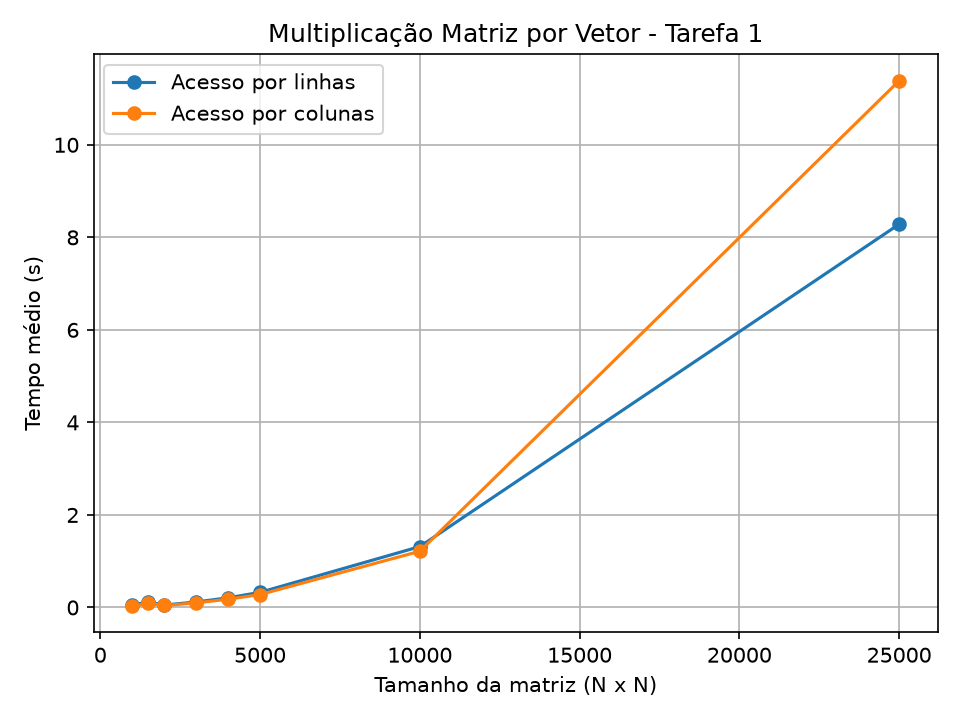
\includegraphics{Graficos/grafico_1}\\
		\par{O gŕafico acima mostra a evolução do tempo de execução de cada método utilizado para essa implementação para matrizes quadradas NxN. Analizando os dados coletados podemos verificar que os tempos de execução permanecem muito próximos para matrizes quadradas com N = 10000, porém rapidamente é percebida uma performance significativamente melhor para o método de acesso por linhas.}
		\par{Esse comportamento se dá pela forma que a linguagem C acessa e armazena dados de matrizes na memória cache. Esse acesso ocorre de forma sequencial, linha por linha. Ou seja, para obter determinado dado em uma matriz a linha completa é salva e percorrida para procurar o dado. Esse comportamento não afeta o método de multiplicação linha por linha, visto que é o comportamento esperado dele: salva a linha, pesquisa o item e já utiliza na multiplicação.}
		\par{Porém, para implementação de coluna por coluna, isso se torna um grande problema para matrizes com linhas muito grandes, pois para cada coluna, mesmo que para obter apenas um item, precisa salvar a linha completa. Ou seja, enquanto o método de linhas precisa salvar a apenas uma vez para buscar o último item da linha, essa versão precisa salvar N linhas para obter o item N dessa coluna.}
		\subsection{CÓDIGO}
		\begin{lstlisting}[language=c]
#define _POSIX_C_SOURCE 200809L

#include <stdio.h>
#include <stdlib.h>
#include <time.h>

double ObterTempoAtual(void)
{
	struct timespec tempo;
	
	clock_gettime(CLOCK_MONOTONIC, &tempo);
	
	return (double)tempo.tv_sec +
	(double)tempo.tv_nsec / 1e9;
}


double *AlocarMatriz(size_t quantidade_linhas, size_t quantidade_colunas)
{
	double *matriz = malloc(quantidade_linhas * quantidade_colunas * sizeof(double));
	if (matriz == NULL)
	{
		fprintf(stderr, "Erro ao alocar matriz.\n");
		exit(EXIT_FAILURE);
	}
	return matriz;
}

double *AlocarVetor(size_t quantidade_elementos)
{
	double *vetor = malloc(quantidade_elementos * sizeof(double));
	if (vetor == NULL)
	{
		fprintf(stderr, "Erro ao alocar vetor.\n");
		exit(EXIT_FAILURE);
	}
	return vetor;
}

void InicializarMatriz(double *matriz, size_t quantidade_linhas, size_t quantidade_colunas)
{
	for (size_t indice_linha = 0; indice_linha < quantidade_linhas; ++indice_linha)
	{
		for (size_t indice_coluna = 0; indice_coluna < quantidade_colunas; ++indice_coluna)
		{
			matriz[indice_linha * quantidade_colunas + indice_coluna] =
			1.0 + (double)((indice_linha + indice_coluna) % 100) / 100.0;
		}
	}
}

void InicializarVetor(double *vetor, size_t quantidade_elementos)
{
	for (size_t indice = 0; indice < quantidade_elementos; ++indice)
	{
		vetor[indice] = 1.0 + (double)(indice % 100) / 100.0;
	}
}

void ZerarVetor(double *vetor, size_t quantidade_elementos)
{
	for (size_t indice = 0; indice < quantidade_elementos; ++indice)
	{
		vetor[indice] = 0.0;
	}
}

void MultiplicarPorLinhas(
const double *matriz,
const double *vetor_entrada,
double *vetor_saida,
size_t quantidade_linhas,
size_t quantidade_colunas)
{
	for (size_t indice_linha = 0; indice_linha < quantidade_linhas; ++indice_linha)
	{
		double soma_linha = 0.0;
		
		for (size_t indice_coluna = 0; indice_coluna < quantidade_colunas; ++indice_coluna)
		{
			soma_linha += matriz[indice_linha * quantidade_colunas + indice_coluna] *
			vetor_entrada[indice_coluna];
		}
		
		vetor_saida[indice_linha] = soma_linha;
	}
}

void MultiplicarPorColunas(
const double *matriz,
const double *vetor_entrada,
double *vetor_saida,
size_t quantidade_linhas,
size_t quantidade_colunas)
{
	ZerarVetor(vetor_saida, quantidade_linhas);
	
	for (size_t indice_coluna = 0; indice_coluna < quantidade_colunas; ++indice_coluna)
	{
		const double valor_vetor_entrada = vetor_entrada[indice_coluna];
		
		for (size_t indice_linha = 0; indice_linha < quantidade_linhas; ++indice_linha)
		{
			vetor_saida[indice_linha] +=
			matriz[indice_linha * quantidade_colunas + indice_coluna] * valor_vetor_entrada;
		}
	}
}
// calcular a diferenca entre as saidas pra ver teve algum erro de calculo entre as matrixes
double CalcularErroMaximo(
const double *primeiro_vetor,
const double *segundo_vetor,
size_t quantidade_elementos)
{
	double maior_erro = 0.0;
	
	for (size_t indice = 0; indice < quantidade_elementos; ++indice)
	{
		double erro_atual = primeiro_vetor[indice] - segundo_vetor[indice];
		if (erro_atual < 0.0)
		{
			erro_atual = -erro_atual;
		}
		if (erro_atual > maior_erro)
		{
			maior_erro = erro_atual;
		}
	}
	
	return maior_erro;
}

double MedirLinhas(
const double *matriz,
const double *vetor_entrada,
double *vetor_saida,
size_t quantidade_linhas,
size_t quantidade_colunas,
size_t repeticoes)
{
	double tempo_inicio = ObterTempoAtual();
	
	for (size_t i = 0; i < repeticoes; ++i)
	{
		MultiplicarPorLinhas(
		matriz, vetor_entrada, vetor_saida, quantidade_linhas, quantidade_colunas);
	}
	
	double tempo_fim = ObterTempoAtual();
	return tempo_fim - tempo_inicio;
}

double MedirColunas(
const double *matriz,
const double *vetor_entrada,
double *vetor_saida,
size_t quantidade_linhas,
size_t quantidade_colunas,
size_t repeticoes)
{
	double tempo_inicio = ObterTempoAtual();
	
	for (size_t i = 0; i < repeticoes; ++i)
	{
		MultiplicarPorColunas(
		matriz, vetor_entrada, vetor_saida, quantidade_linhas, quantidade_colunas);
	}
	
	double tempo_fim = ObterTempoAtual();
	return tempo_fim - tempo_inicio;
}

/* Executa um teste para uma matriz quadrada n x n. */
void ExecutarTeste(size_t repeticoes, size_t tamanho_matriz, FILE *arquivo_saida)
{
	double *matriz = AlocarMatriz(tamanho_matriz, tamanho_matriz);
	double *vetor_entrada = AlocarVetor(tamanho_matriz);
	double *vetor_saida_linhas = AlocarVetor(tamanho_matriz);
	double *vetor_saida_colunas = AlocarVetor(tamanho_matriz);
	
	InicializarMatriz(matriz, tamanho_matriz, tamanho_matriz);
	InicializarVetor(vetor_entrada, tamanho_matriz);
	
	double tempo_linhas = MedirLinhas(
	matriz, vetor_entrada, vetor_saida_linhas, tamanho_matriz, tamanho_matriz, repeticoes);
	
	double tempo_colunas = MedirColunas(
	matriz, vetor_entrada, vetor_saida_colunas, tamanho_matriz, tamanho_matriz, repeticoes);
	
	double erro_maximo = CalcularErroMaximo(
	vetor_saida_linhas, vetor_saida_colunas, tamanho_matriz);
	
	fprintf(arquivo_saida, "%zu,%zu,%.12f,%.12f,%.12e\n",
	tamanho_matriz, repeticoes, tempo_linhas, tempo_colunas, erro_maximo);
	
	printf("N=%zu | linhas=%.6f s | colunas=%.6f s | erro=%.3e\n",
	tamanho_matriz, tempo_linhas, tempo_colunas, erro_maximo);
	
	free(matriz);
	free(vetor_entrada);
	free(vetor_saida_linhas);
	free(vetor_saida_colunas);
}

int main(void)
{
	const size_t tamanhos_matriz[] = {1000, 1500, 2000, 3000, 4000, 5000, 10000, 25000};
	
	const size_t quantidade_tamanhos =
	sizeof(tamanhos_matriz) / sizeof(tamanhos_matriz[0]);
	
	// arquivo pra plotar graficos com python pro relatorio
	FILE *arquivo_saida = fopen("resultados.csv", "w");
	if (arquivo_saida == NULL)
	{
		fprintf(stderr, "Erro ao criar resultados.csv.\n");
		return EXIT_FAILURE;
	}
	
	fprintf(arquivo_saida,
	"tamanho,repeticoes,tempo_linhas_s,tempo_colunas_s,erro_maximo\n");
	
	for (size_t indice_tamanho = 0; indice_tamanho < quantidade_tamanhos; ++indice_tamanho)
	{
		size_t n = tamanhos_matriz[indice_tamanho];
		
		int repeticoes;
		if (n <= 500)
		{
			repeticoes = 100;
		}
		else if (n <= 1500)
		{
			repeticoes = 20;
		}
		else
		{
			repeticoes = 5;
		}
		
		ExecutarTeste(repeticoes, n, arquivo_saida);
	}
	
	fclose(arquivo_saida);
	
	printf("\nResultados salvos em resultados.csv\n");
	
	return EXIT_SUCCESS;
}
		\end{lstlisting}
	
	\newpage
		\onehalfspacing
		\section{TAREFA 2}
		\subsection{\subtUm}
		\par{Implementar a soma dos itens de um vetor qualquer de forma cumulativa, de forma que exista dependência entres as iterações, usando variáveis auxiliares para quebrar essa dependência. Utilizar diferentes níveis de otimização e diferentes tamanhos do vetor para comparar a performance entre cada versão, analisando como as dependências afetam o desempenho e quais as otimizações executadas pelo compilador.}
		\subsection{\subtDois}
		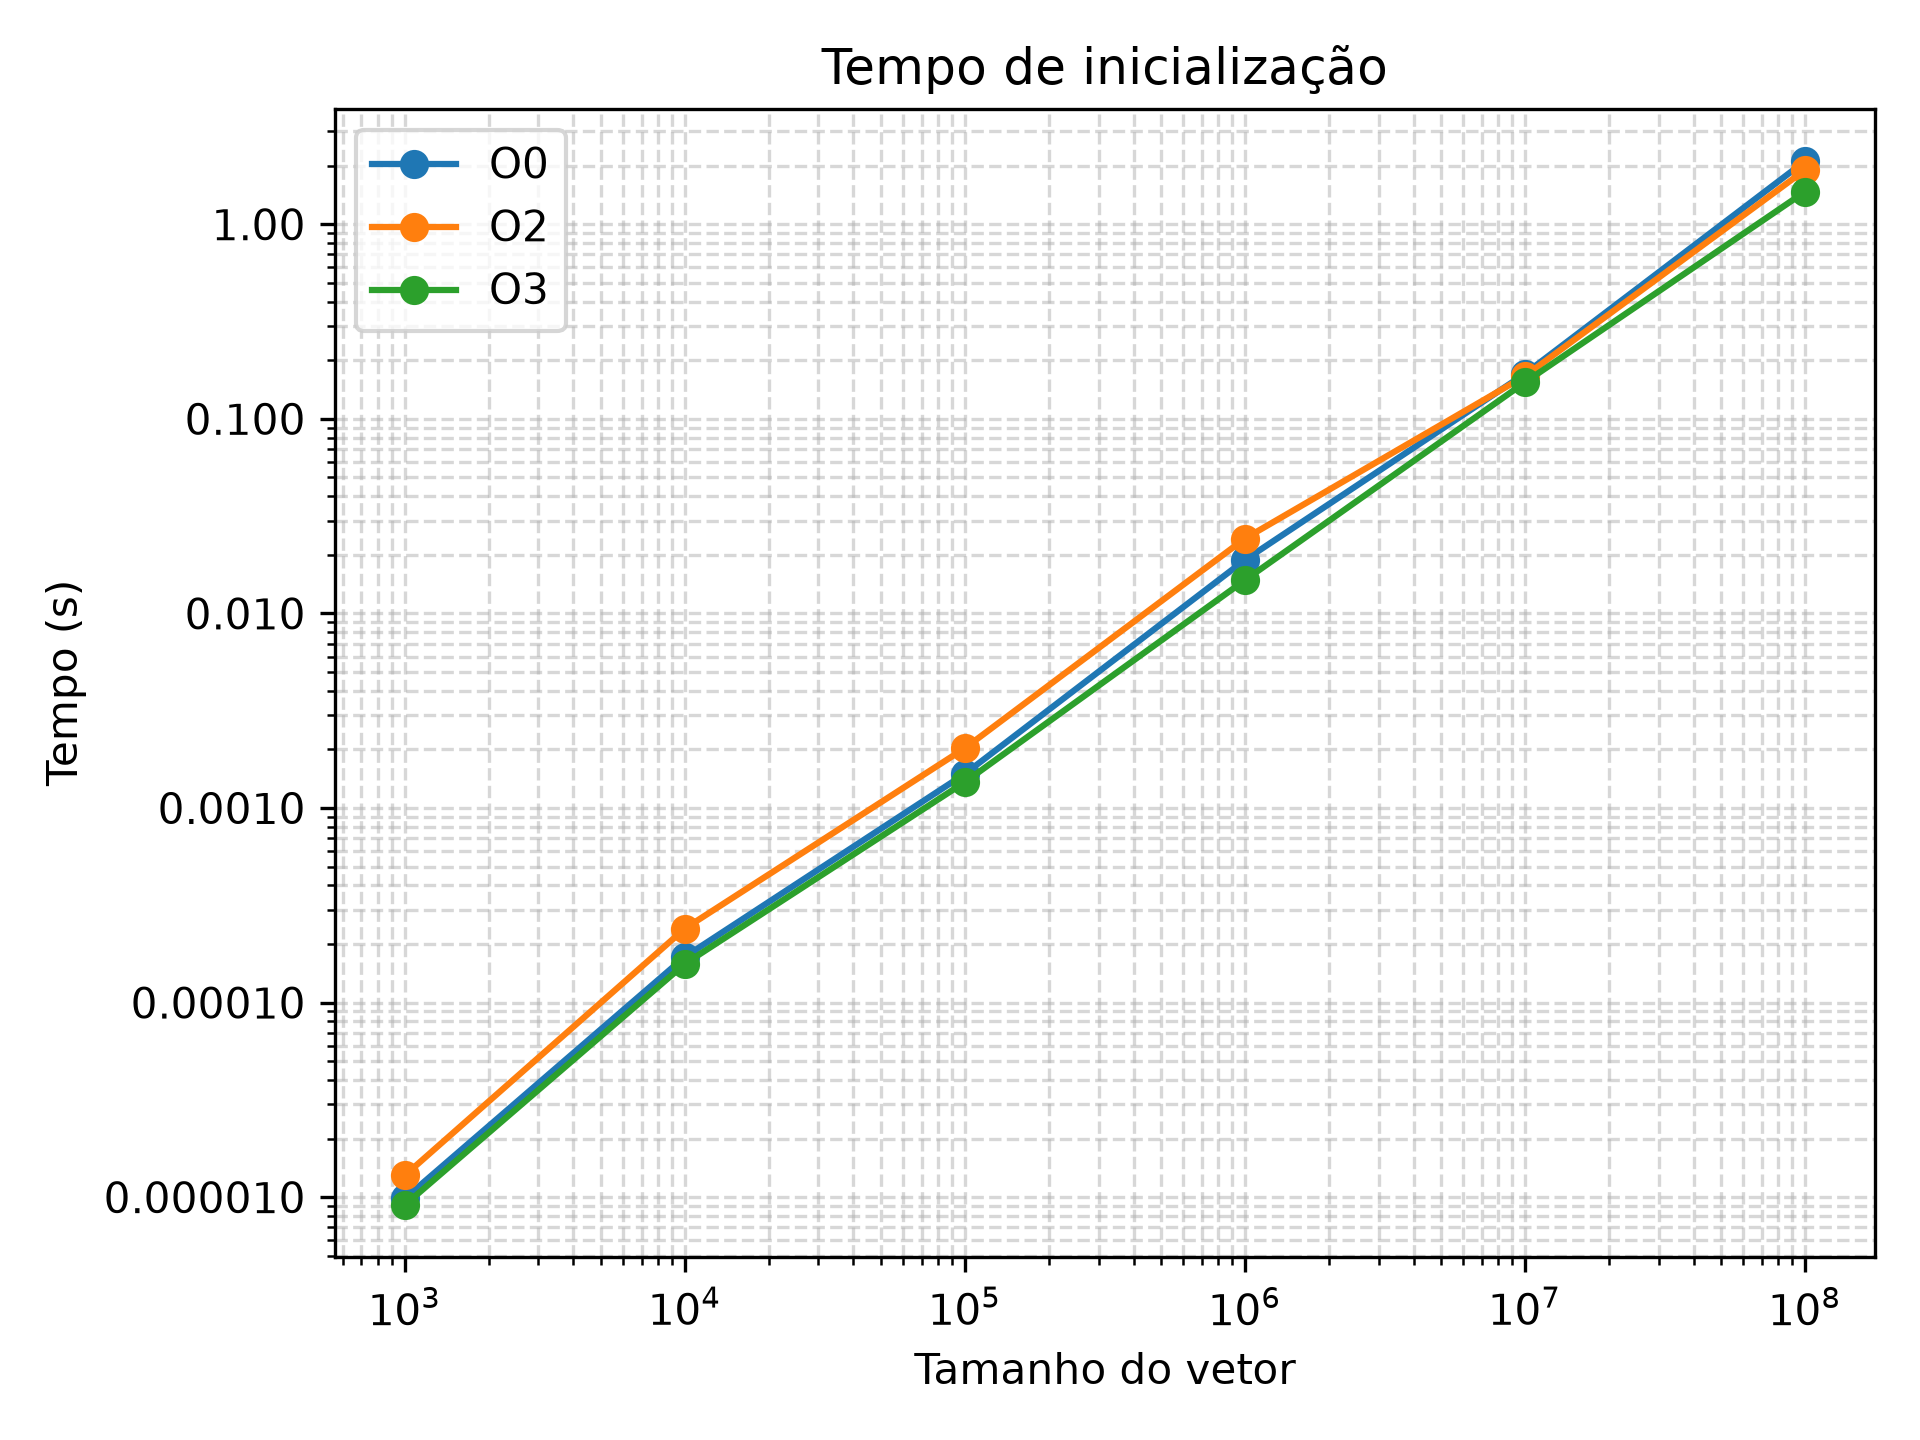
\includegraphics{Tarefa2/inicializacao.png}\\
		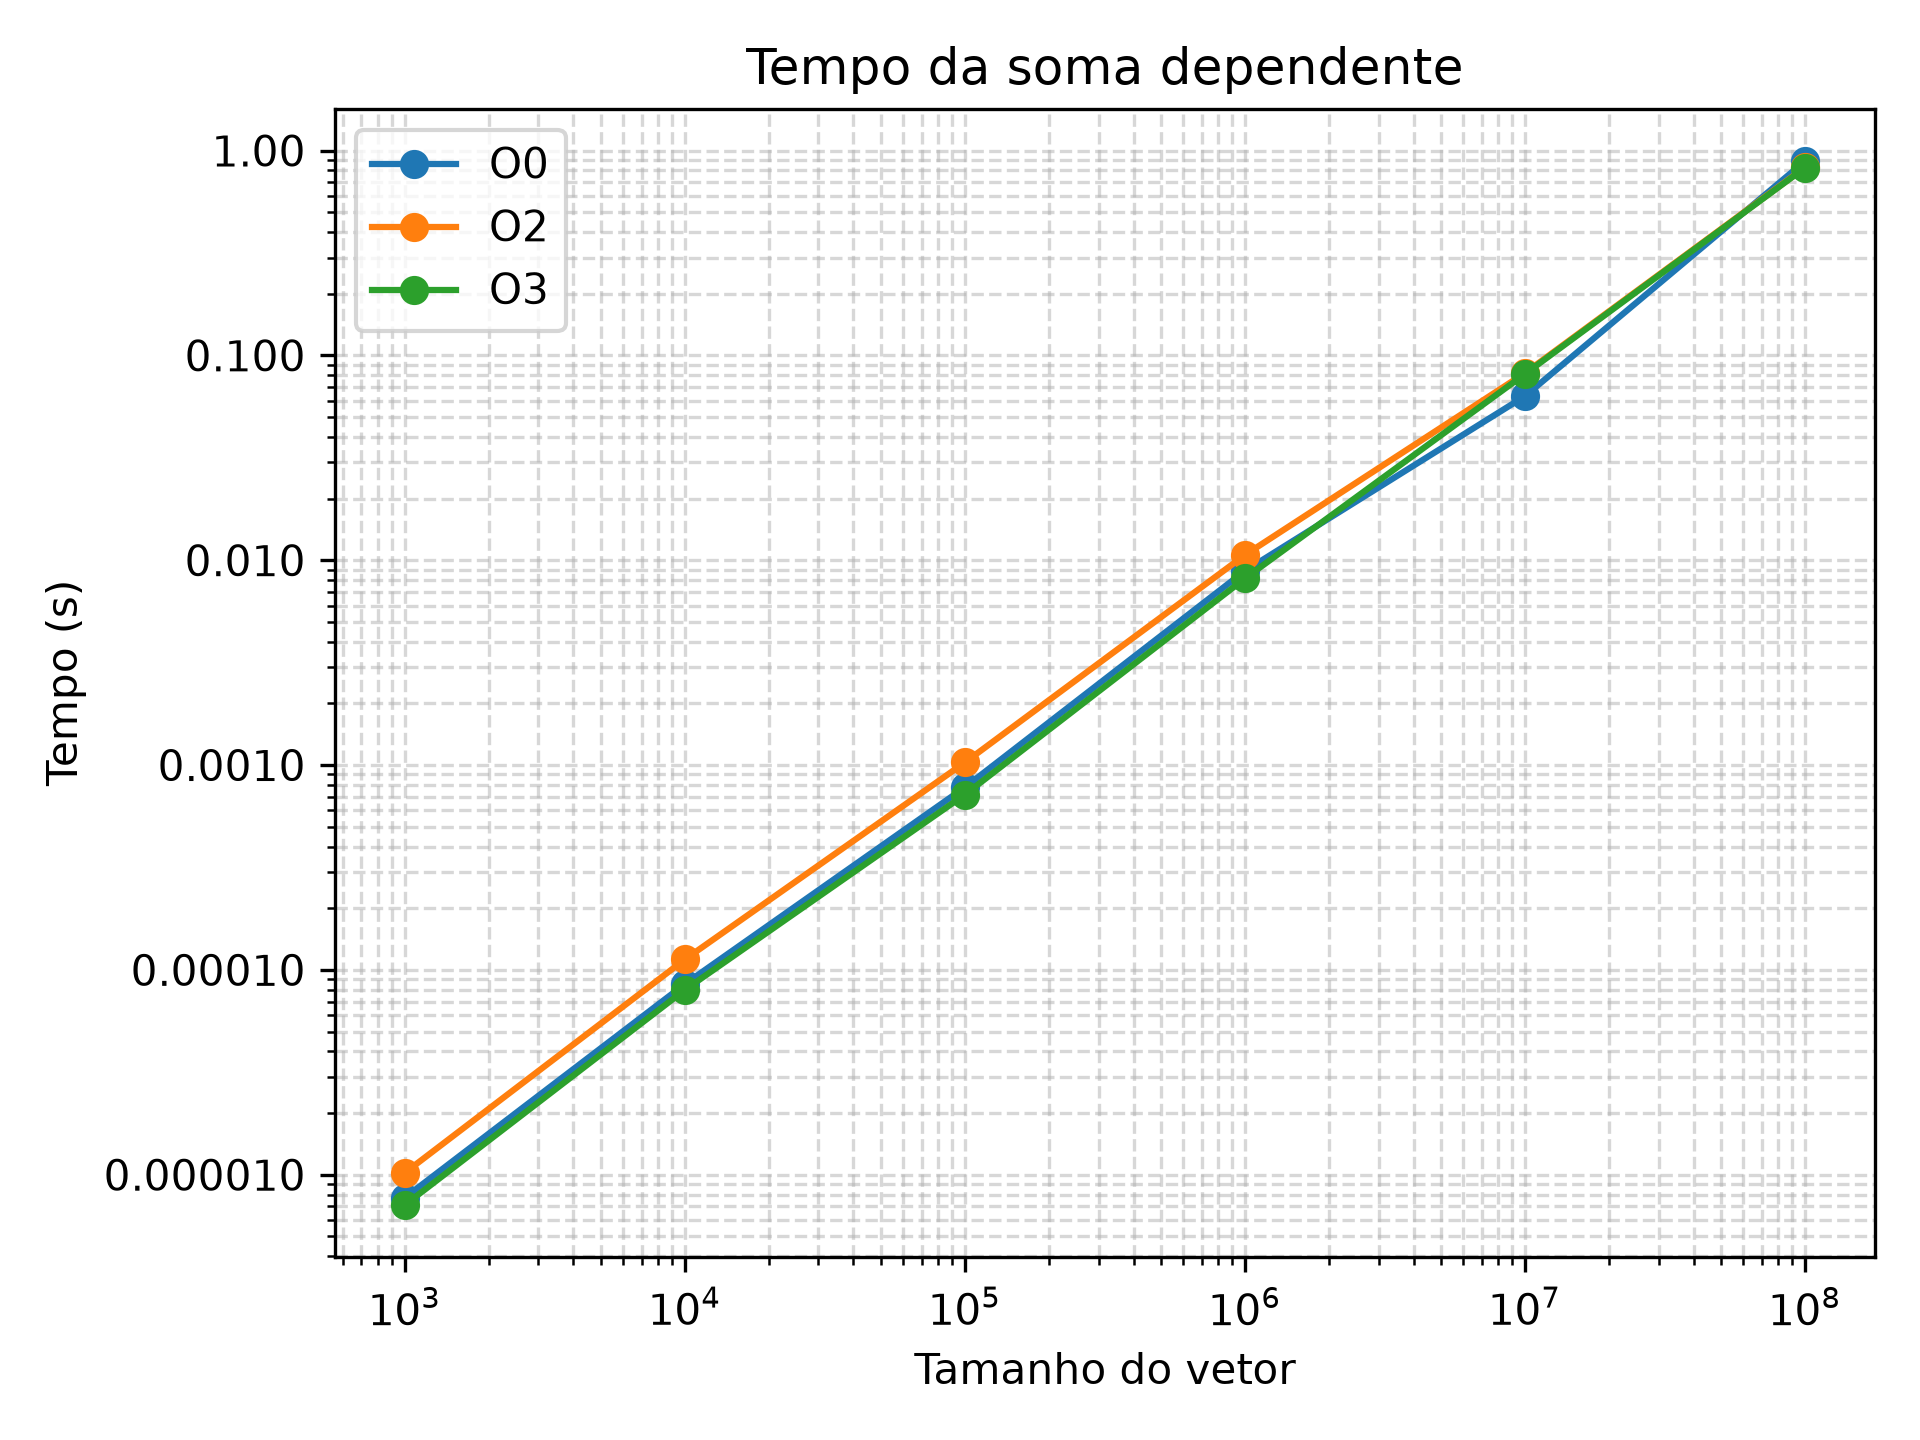
\includegraphics{Tarefa2/soma_dependente.png}\\
		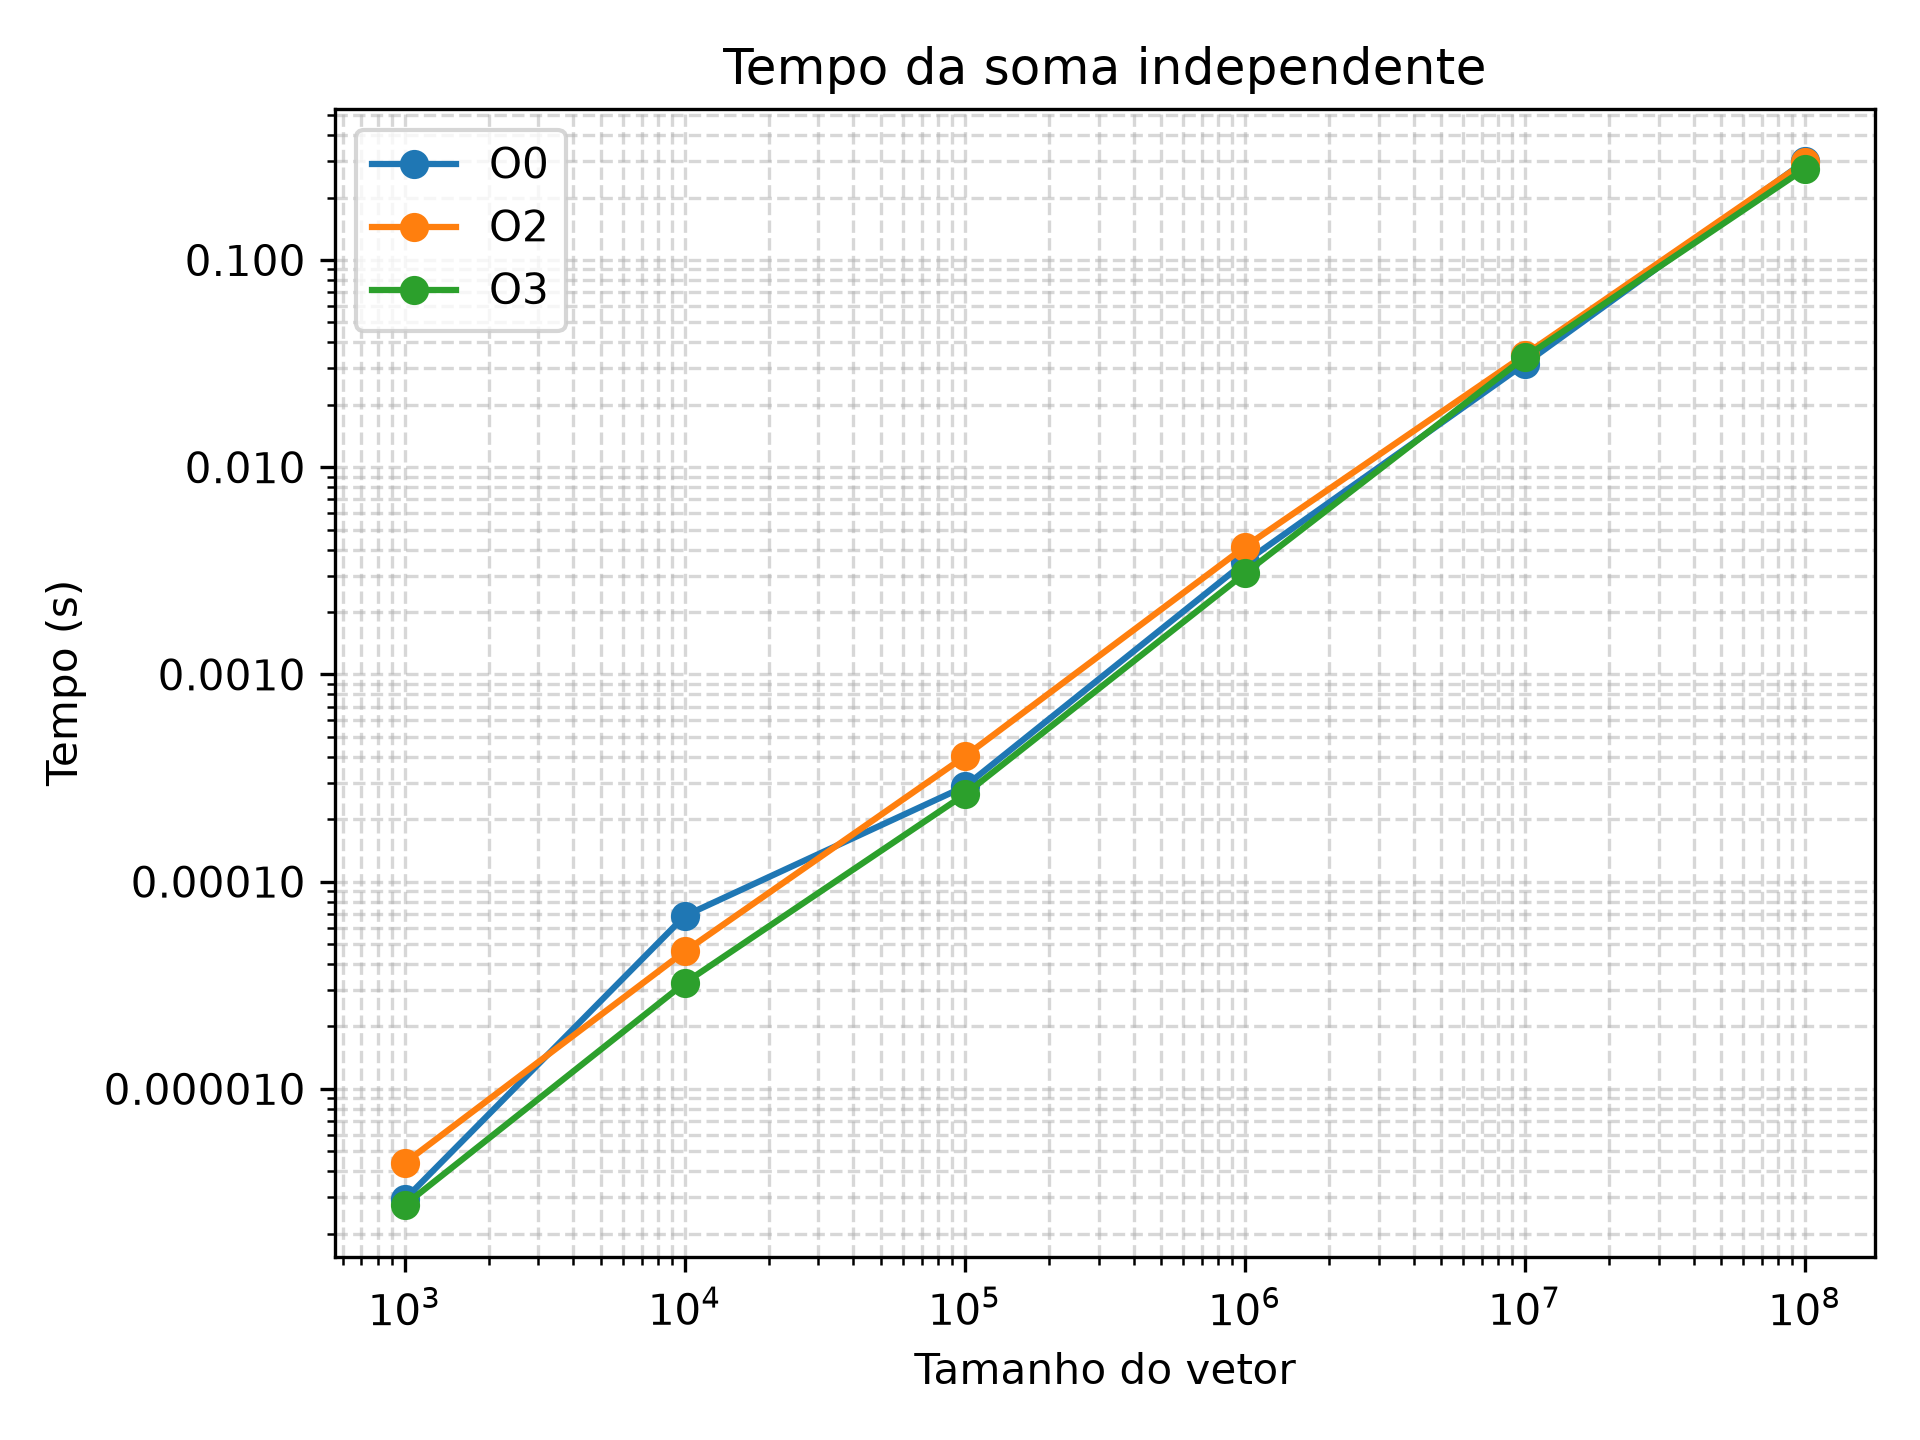
\includegraphics{Tarefa2/soma_independente.png}\\
		\par{Analisando os números obtidos, verificamos que a estrutura do código e as dependências têm influência direta em quanto o compilador consegue otimizar a execução.}
		\par{A soma dependente tem uma cadeia de dependência entre suas iterações, limitando o paralelismo e fazendo com ue O2 e O3 tenham desempenho relativamente próximo ao de OO. Já a soma independente utiliza quatro acumuladores,  que elimina essa dependência e permite maior aproveitamento do paralelismo, tendo desempenho significativamente melhor.}
		\par{As versões O2 e O3 também apresentaram melhora na inicialização do programa, além da soma independente. Porém esses ganhos não são ilimitados, pois o programa também é limitado pelo acesso a memória e performance geral da máquina usada nos testes, o que faz com que a performance quase equalize em certos pontos.}
		\subsection{CÓDIGO}
		\begin{lstlisting}[language=c]
#include <stdint.h>
#include <stdio.h>
#include <stdlib.h>
#include <time.h>

typedef struct {
	double inicializacao;
	double soma_dependente;
	double soma_independente;
} Resultado;

double obter_tempo_atual(void) {
	struct timespec tempo;
	
	clock_gettime(CLOCK_MONOTONIC, &tempo);
	
	return (double)tempo.tv_sec + (double)tempo.tv_nsec / 1e9;
}

double *criar_vetor(size_t tamanho) {
	double *vetor = malloc(tamanho * sizeof(double));
	
	if (vetor == NULL) {
		fprintf(stderr, "Erro ao alocar vetor\n");
		exit(EXIT_FAILURE);
	}
	
	return vetor;
}

void liberar_vetor(double *vetor) { free(vetor); }

void inicializar_vetor(double *vetor, size_t tamanho) {
	for (size_t i = 0; i < tamanho; i++) {
		vetor[i] = (double)i * 1.5 + 10.0;
	}
}

double somar_dependente(const double *vetor, size_t tamanho) {
	double soma = 0.0;
	
	for (size_t i = 0; i < tamanho; i++) {
		soma += vetor[i];
	}
	
	return soma;
}

double somar_independente(const double *vetor, size_t tamanho) {
	double soma1 = 0.0;
	double soma2 = 0.0;
	double soma3 = 0.0;
	double soma4 = 0.0;
	
	size_t i = 0;
	
	for (; i + 3 < tamanho; i += 4) {
		soma1 += vetor[i];
		soma2 += vetor[i + 1];
		soma3 += vetor[i + 2];
		soma4 += vetor[i + 3];
	}
	
	for (; i < tamanho; i++) {
		soma1 += vetor[i];
	}
	
	return soma1 + soma2 + soma3 + soma4;
}

double medir_inicializacao(double *vetor, size_t tamanho) {
	double inicio = obter_tempo_atual();
	
	inicializar_vetor(vetor, tamanho);
	
	double fim = obter_tempo_atual();
	
	return fim - inicio;
}

double medir_soma_dependente(const double *vetor, size_t tamanho,
double *resultado) {
	double inicio = obter_tempo_atual();
	
	*resultado = somar_dependente(vetor, tamanho);
	
	double fim = obter_tempo_atual();
	
	return fim - inicio;
}

double medir_soma_independente(const double *vetor, size_t tamanho,
double *resultado) {
	double inicio = obter_tempo_atual();
	
	*resultado = somar_independente(vetor, tamanho);
	
	double fim = obter_tempo_atual();
	
	return fim - inicio;
}

Resultado executar_testes(size_t tamanho) {
	Resultado resultado;
	double soma_dependente;
	double soma_independente;
	
	double *vetor = criar_vetor(tamanho);
	
	resultado.inicializacao = medir_inicializacao(vetor, tamanho);
	
	resultado.soma_dependente =
	medir_soma_dependente(vetor, tamanho, &soma_dependente);
	
	resultado.soma_independente =
	medir_soma_independente(vetor, tamanho, &soma_independente);
	
	printf("%zu,%.9f,%.9f,%.9f,%.2f,%.2f\n", tamanho, resultado.inicializacao,
	resultado.soma_dependente, resultado.soma_independente,
	soma_dependente, soma_independente);
	
	liberar_vetor(vetor);
	
	return resultado;
}

void executar_tamanhos(const size_t *tamanhos, size_t quantidade) {
	for (size_t i = 0; i < quantidade; i++) {
		executar_testes(tamanhos[i]);
	}
}

int main(void) {
	const size_t tamanhos[] = {1000, 10000, 100000, 1000000, 10000000, 100000000};
	
	size_t quantidade = sizeof(tamanhos) / sizeof(tamanhos[0]);
	
	printf("tamanho,inicializacao,soma_dependente,"
	"soma_independente,resultado_dependente,"
	"resultado_independente\n");
	
	executar_tamanhos(tamanhos, quantidade);
	
	return 0;
}
		\end{lstlisting}
	
	\newpage
		\onehalfspacing
		\section{TAREFA 3}
		\subsection{\subtUm}
		\par{Dados dois códigos, analisar e explicar o comportamento observado na variável de saída "contador", identificando a origem a dos problemas e apresentando soluções para os erros, discutindo os conceitos de processo e thread e comparando seus funcionamentos, especialmente em relação a compartilhamento de memória e programação concorrente.}
		\subsection{\subtDois}
		\par{
		No primeiro código disponibilizado, como os processos são uma "cópia" do código pai rodando separadamente, com sua própria memória, todos iniciam com o contador = 0. Dessa forma, cada um realiza sua própria soma até que contador = 1000000, e, ao retornar, o pai ainda terá contador = 0. Como a intenção seja somar todos em 'contador', para atingir esse objetivo podemos usar semáforos para acessar uma memória compartilhada entre os filhos, que poderia ser acessada também pelo pai. Essa versão corrigida está na parte de códigos dessa seção.
		}
		\par{
		Já o segundo código apresenta um problema de região crítica no acesso à variável contador:
		}
		\begin{lstlisting}[language=c]
int contador = 0;
void *incrementar(void *arg)
{
	for (int i = 0; i < INCREMENTOS; i++)
	{
		contador++;
	}
	return NULL;
}
// [...]
int erro = pthread_create( threads[i], NULL, incrementar, NULL);
// [...]
		\end{lstlisting}
		\par{
		Como todas as threads atuam ao mesmo tempo, todas recebem o mesmo valor de contador antes de realizarem sua ação (nesse caso, contador++). Assim, caso fiquem todas alinhadas no tempo, contador finalizaria com o valor 1000000, porém na realidade acontecem pequenas variações onde threads finalizam antes das outras iniciarem, fazendo o código terminar com um valor aleatoriamente maior. Para corrigir poderíamos alterar o programa para permitir acesso à variável uma thread por vez usando mutex, "travando" a variável antes e destravando depois na função incrementar. A versão corrigida está na parte de códigos dessa seção.
		}
		\subsection{\subtTres}
		\begin{lstlisting}[language=c]
// CONT1.C - CORRIGIDO COM SEMAFOROS

#include <stdio.h>
#include <stdlib.h>
#include <unistd.h>
#include <sys/wait.h>
#include <sys/mman.h>
#include <semaphore.h>

#define NUM_PROCESSOS 4
#define INCREMENTOS 1000000

int main()
{
	int *contador = mmap(NULL, sizeof(int), PROT_READ | PROT_WRITE, MAP_SHARED | MAP_ANONYMOUS, -1, 0);
	if (contador == MAP_FAILED)
	{
		perror("Erro ao criar memoria compartilhada");
		exit(EXIT_FAILURE);
	}
	*contador = 0;
	
	// semaforo compartilhado entre processos
	sem_t *sem = mmap(NULL, sizeof(sem_t), PROT_READ | PROT_WRITE,
	MAP_SHARED | MAP_ANONYMOUS, -1, 0);
	if (sem == MAP_FAILED)
	{
		perror("Erro ao criar semaforo");
		exit(EXIT_FAILURE);
	}
	sem_init(sem, 1, 1);
	
	printf("Contador inicial: %d\n", *contador);
	
	for (int i = 0; i < NUM_PROCESSOS; i++)
	{
		pid_t pid = fork();
		if (pid < 0)
		{
			perror("Erro ao criar processo");
			exit(EXIT_FAILURE);
		}
		if (pid == 0)
		{
			// Codigo executado pelo processo filho
			for (int j = 0; j < INCREMENTOS; j++)
			{
				sem_wait(sem); // trava
				(*contador)++;
				sem_post(sem); // destrava
			}
			printf("Filho %d terminou\n", getpid());
			exit(EXIT_SUCCESS);
		}
	}
	
	// Processo pai espera todos os filhos
	for (int i = 0; i < NUM_PROCESSOS; i++)
	{
		wait(NULL);
	}
	
	printf("\nContador no processo pai: %d\n", *contador);
	
	// Limpeza
	sem_destroy(sem);
	munmap(contador, sizeof(int));
	munmap(sem, sizeof(sem_t));
	
	return 0;
}
		\end{lstlisting}
		\begin{lstlisting}
// CONT2.C - VERSAO CORRIGIDA

#include <stdio.h>
#include <stdlib.h>
#include <pthread.h>

#define NUM_THREADS 4
#define INCREMENTOS 1000000

int contador = 0;
pthread_mutex_t mutex = PTHREAD_MUTEX_INITIALIZER;

void *incrementar(void *arg)
{
	for (int i = 0; i < INCREMENTOS; i++)
	{
		pthread_mutex_lock(&mutex);
		contador++;
		pthread_mutex_unlock(&mutex);
	}
	return NULL;
}

int main()
{
	pthread_t threads[NUM_THREADS];
	printf("Contador inicial: %d\n", contador);
	// Criar as threads
	for (int i = 0; i < NUM_THREADS; i++)
	{
		int erro = pthread_create(
		&threads[i],
		NULL,
		incrementar,
		NULL);
		if (erro != 0)
		{
			fprintf(stderr, "Erro ao criar thread\n");
			exit(EXIT_FAILURE);
		}
	}
	// Esperar todas as threads
	for (int i = 0; i < NUM_THREADS; i++)
	{
		pthread_join(threads[i], NULL);
	}
	printf("\nContador final: %d\n", contador);
	
	pthread_mutex_destroy(&mutex);
	return 0;
}
		\end{lstlisting}
	\newpage
		\onehalfspacing
		\section{TAREFA 4}
		\subsection{\subtUm}
		\par{Implementar uma versão sequencial do calculo de integrais definidas utilizando o método do trapézio. Analisar o código e discutir sobre o resultado encontrado, quais partes podem ser paralelizadas e os possíveis desafios e problemas encontrados ao tentar implementar uma versão de cálculo paralelo.
		}
		\subsection{\subtDois}
		\par{A parte principal a ser paralelizada é a função \texttt{calcular\_soma()}, pois utiliza um laço de repetição em que as iterações independem umas das outras, permitindo a paralelização e um ganho significativo de desempenho.}
		\par{Caso esse código fosse somente paralelizado, porém, encontraria um problema de condição de corrida na variável \texttt{soma} utilizada para guardar o resultado, visto que as threads iriam acessar e alterar simultaneamente o mesmo local, causando um resultado inconsistente.}
		\par{Portanto seria necessário implementar uma técnica de sincronização, usando semáforos para que cada uma tenha acesso a ela de cada vez, ou preferencialmente usando redução. Como é um problema simples de soma, podemos definir uma soma parcial para cada thread, que será somada ao resultado total ao fim do cálculo.}
		\subsection{\subtTres}
		\begin{lstlisting}[language=c]
#include <stdio.h>
#include <stdlib.h>
#include <math.h>

double funcao(double x)
{
	return x * x;
}

double calcular_passo(double a, double b, int n)
{
	return (b - a) / n;
}

double calcular_soma(double a, double h, int n)
{
	double soma = 0.0;
	
	for (int i = 1; i < n; i++)
	{
		double x = a + i * h;
		soma += funcao(x);
	}
	
	return soma;
}

double calcular_integral(double a, double b, int n)
{
	double h = calcular_passo(a, b, n);
	
	double soma = calcular_soma(a, h, n);
	
	return h * (funcao(a) / 2.0 + funcao(b) / 2.0 + soma);
}

int main(void)
{
	double a;
	double b;
	int n;
	
	printf("Digite o limite inferior a: ");
	scanf("%lf", &a);
	
	printf("Digite o limite superior b: ");
	scanf("%lf", &b);
	
	printf("Digite o numero de subdivisoes n: ");
	scanf("%d", &n);
	
	if (n <= 0 || a >= b)
	{
		printf("Valores invalidos.\n");
		return EXIT_FAILURE;
	}
	
	double resultado = calcular_integral(a, b, n);
	// formula da integral exata pra x^2
	double exato = (pow(b, 3) - pow(a, 3)) / 3.0;
	
	printf("\nIntegral aproximada (trapezio): %.10f\n", resultado);
	printf("Integral exata: %.10f\n", exato);
	printf("Erro: %.10f\n", fabs(resultado - exato));
	
	return EXIT_SUCCESS;
}
		\end{lstlisting}
		
	\newpage
		\onehalfspacing
		\section{TAREFA 5}
		\subsection{\subtUm}
		\par{Implementar um contador de números primos entre 2 e um valor máximo n, paralelizar com a diretiva dada e comparar os resultados das versões sequenciais e paralelas, observando possíveis diferenças no resultado e desempenho. Analisar desafios iniciais da programação paralela como correção e distribuição de carga}
		\subsection{\subtDois}
		\begin{figure}[htbp]
			\centering
			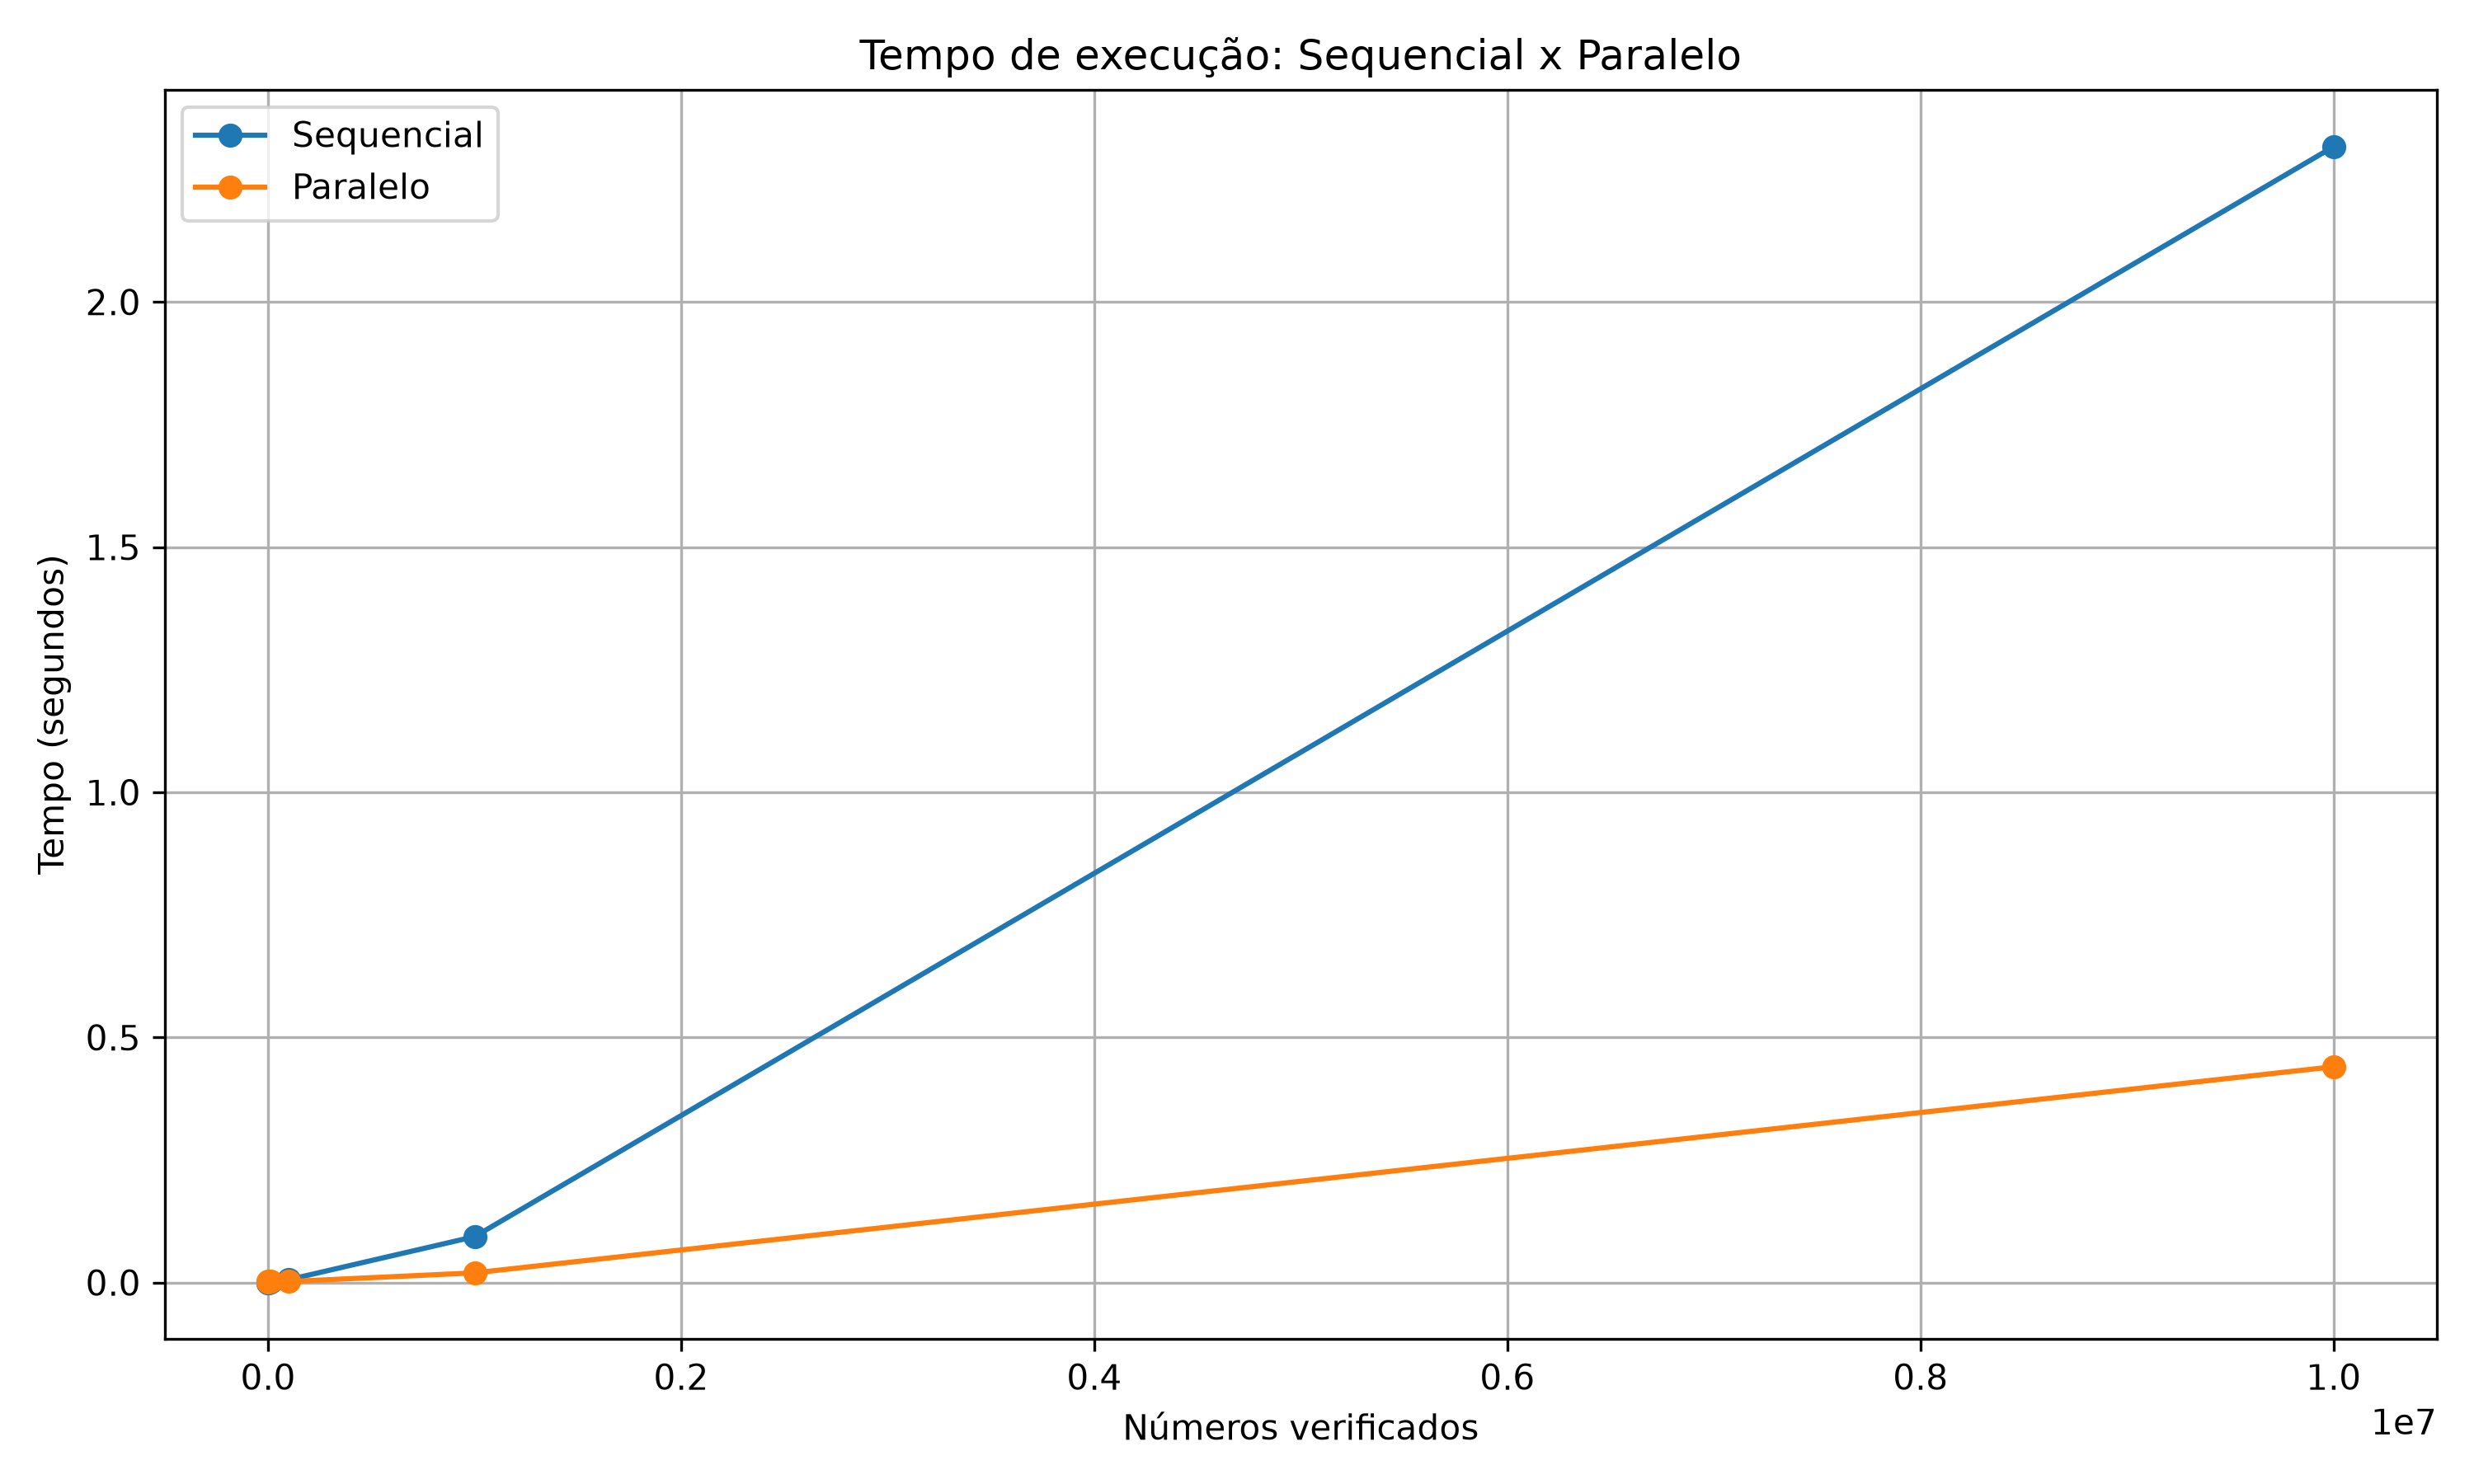
\includegraphics[width=1\textwidth]{Tarefa5/tarefa5.png}
		\end{figure}
		\par{Analisando o gráfico é possível verificar que a versão paralelizada tem um desempenho consideravelmente melhor do que a versão sequencial para números grandes, enquanto que para números pequenos a performance pode ser igual ou pior, a depender do overhead de inicilização.}
		\par{Os desafios encontrados ao transformar a versão sequencial em uma versão paralelizada se devem ao acesso à variável de resultado, visto que na paralelização ela seria uma região crítica, e por isso foi necessário trabalhar com a diretiva \texttt{reduction} para permitir a soma corretamente de cada thread.}
		\par{Além disso, há o problema da distribuição de carga, corrigido pela diretiva \texttt{\#pragma omp parallel for}, que distribui automaticamente as iterações dos laços entre as threads. A função de checagem \texttt{isPrimo()} pode executar diferentes quantidades de operações dependendo do número analisado, desbalanceando a carga de trabalho das threads, por isso foi necessário implementar a correção.}
		\subsection{\subtTres}
		\begin{lstlisting}[language=c]
\#include <omp.h>
\#include <stdbool.h>
\#include <stdio.h>

bool isPrimo(int numero) \{
if (numero < 2) \{
return false;
\}

for (int i = 2; i * i <= numero; i++) \{
if (numero \% i == 0) \{
return false;
\}
\}

return true;
\}

double contarSequencial(int num\_inicio, int num\_fim) \{
int numeros\_verificados = num\_fim - num\_inicio;
int primos\_encontrados = 0;

double tempo\_i = omp\_get\_wtime();

for (int i = num\_inicio + 1; i < num\_fim; i++) \{
if (isPrimo(i)) \{
primos\_encontrados++;
\}
\}

double tempo\_f = omp\_get\_wtime();
double tempo\_gasto = tempo\_f - tempo\_i;

printf(``[SEQ] | \# Verificados: \%d | Primos: \%d | Tempo: \%f\textbackslash{}n'',
numeros\_verificados, primos\_encontrados, tempo\_gasto);

return tempo\_gasto;
\}

double contarParalelo(int num\_inicio, int num\_fim) \{
int numeros\_verificados = num\_fim - num\_inicio;
int primos\_encontrados = 0;

double tempo\_i = omp\_get\_wtime();

\#pragma omp parallel for reduction(+ : primos\_encontrados)
for (int i = num\_inicio + 1; i < num\_fim; i++) \{
if (isPrimo(i)) \{
primos\_encontrados++;
\}
\}

double tempo\_f = omp\_get\_wtime();
double tempo\_gasto = tempo\_f - tempo\_i;

printf(``[PAR] | \# Verificados: \%d | Primos: \%d | Tempo: \%f\textbackslash{}n'',
numeros\_verificados, primos\_encontrados, tempo\_gasto);

return tempo\_gasto;
\}

int main() \{
int inicio = 2;

const size\_t iteracoes[] = \{100, 1000, 10000, 100000, 1000000, 10000000\};

const size\_t quantidade = sizeof(iteracoes) / sizeof(iteracoes[0]);

FILE *arquivo\_saida = fopen("resultados5.csv'', "w'');

if (arquivo\_saida == NULL) \{
printf("Erro ao abrir o arquivo CSV.\textbackslash{}n'');
return 1;
\}

// Cabeçalho do CSV
fprintf(arquivo\_saida,
``numeros\_verificados,tempo\_sequencial,tempo\_paralelo\textbackslash{}n'');

for (size\_t i = 0; i < quantidade; i++) \{
int fim = iteracoes[i];

printf(``\n====== BUSCANDO PRIMOS ATÉ \%d ======\n'', fim);

double tempo\_sequencial = contarSequencial(inicio, fim);
double tempo\_paralelo = contarParalelo(inicio, fim);

fprintf(arquivo\_saida, ``\%d,\%f,\%f\textbackslash{}n'', fim - inicio, tempo\_sequencial,
tempo\_paralelo);
\}

fclose(arquivo\_saida);

printf(``\textbackslash{}nResultados salvos em resultados5.csv\textbackslash{}n'');

return 0;
\}
		\end{lstlisting}
	
	\newpage
		\onehalfspacing
		\section{TAREFA 6}
		\subsection{\subtUm}
			\par{Implementar diversas versões de um programa para cálculo de integrais definidas utilizando o método do trapézio para uma função f(x) num intervalo [a,b], utilizando n subdivisões. Comparar os resultados obtidos e tempos médios de execução com base no crescimento de n. Discutir a corretude dos dados, diferenças entre as versões, diferenças de desempenho, etc.}
		\subsection{\subtDois}
			\begin{figure}[H]
				\centering
				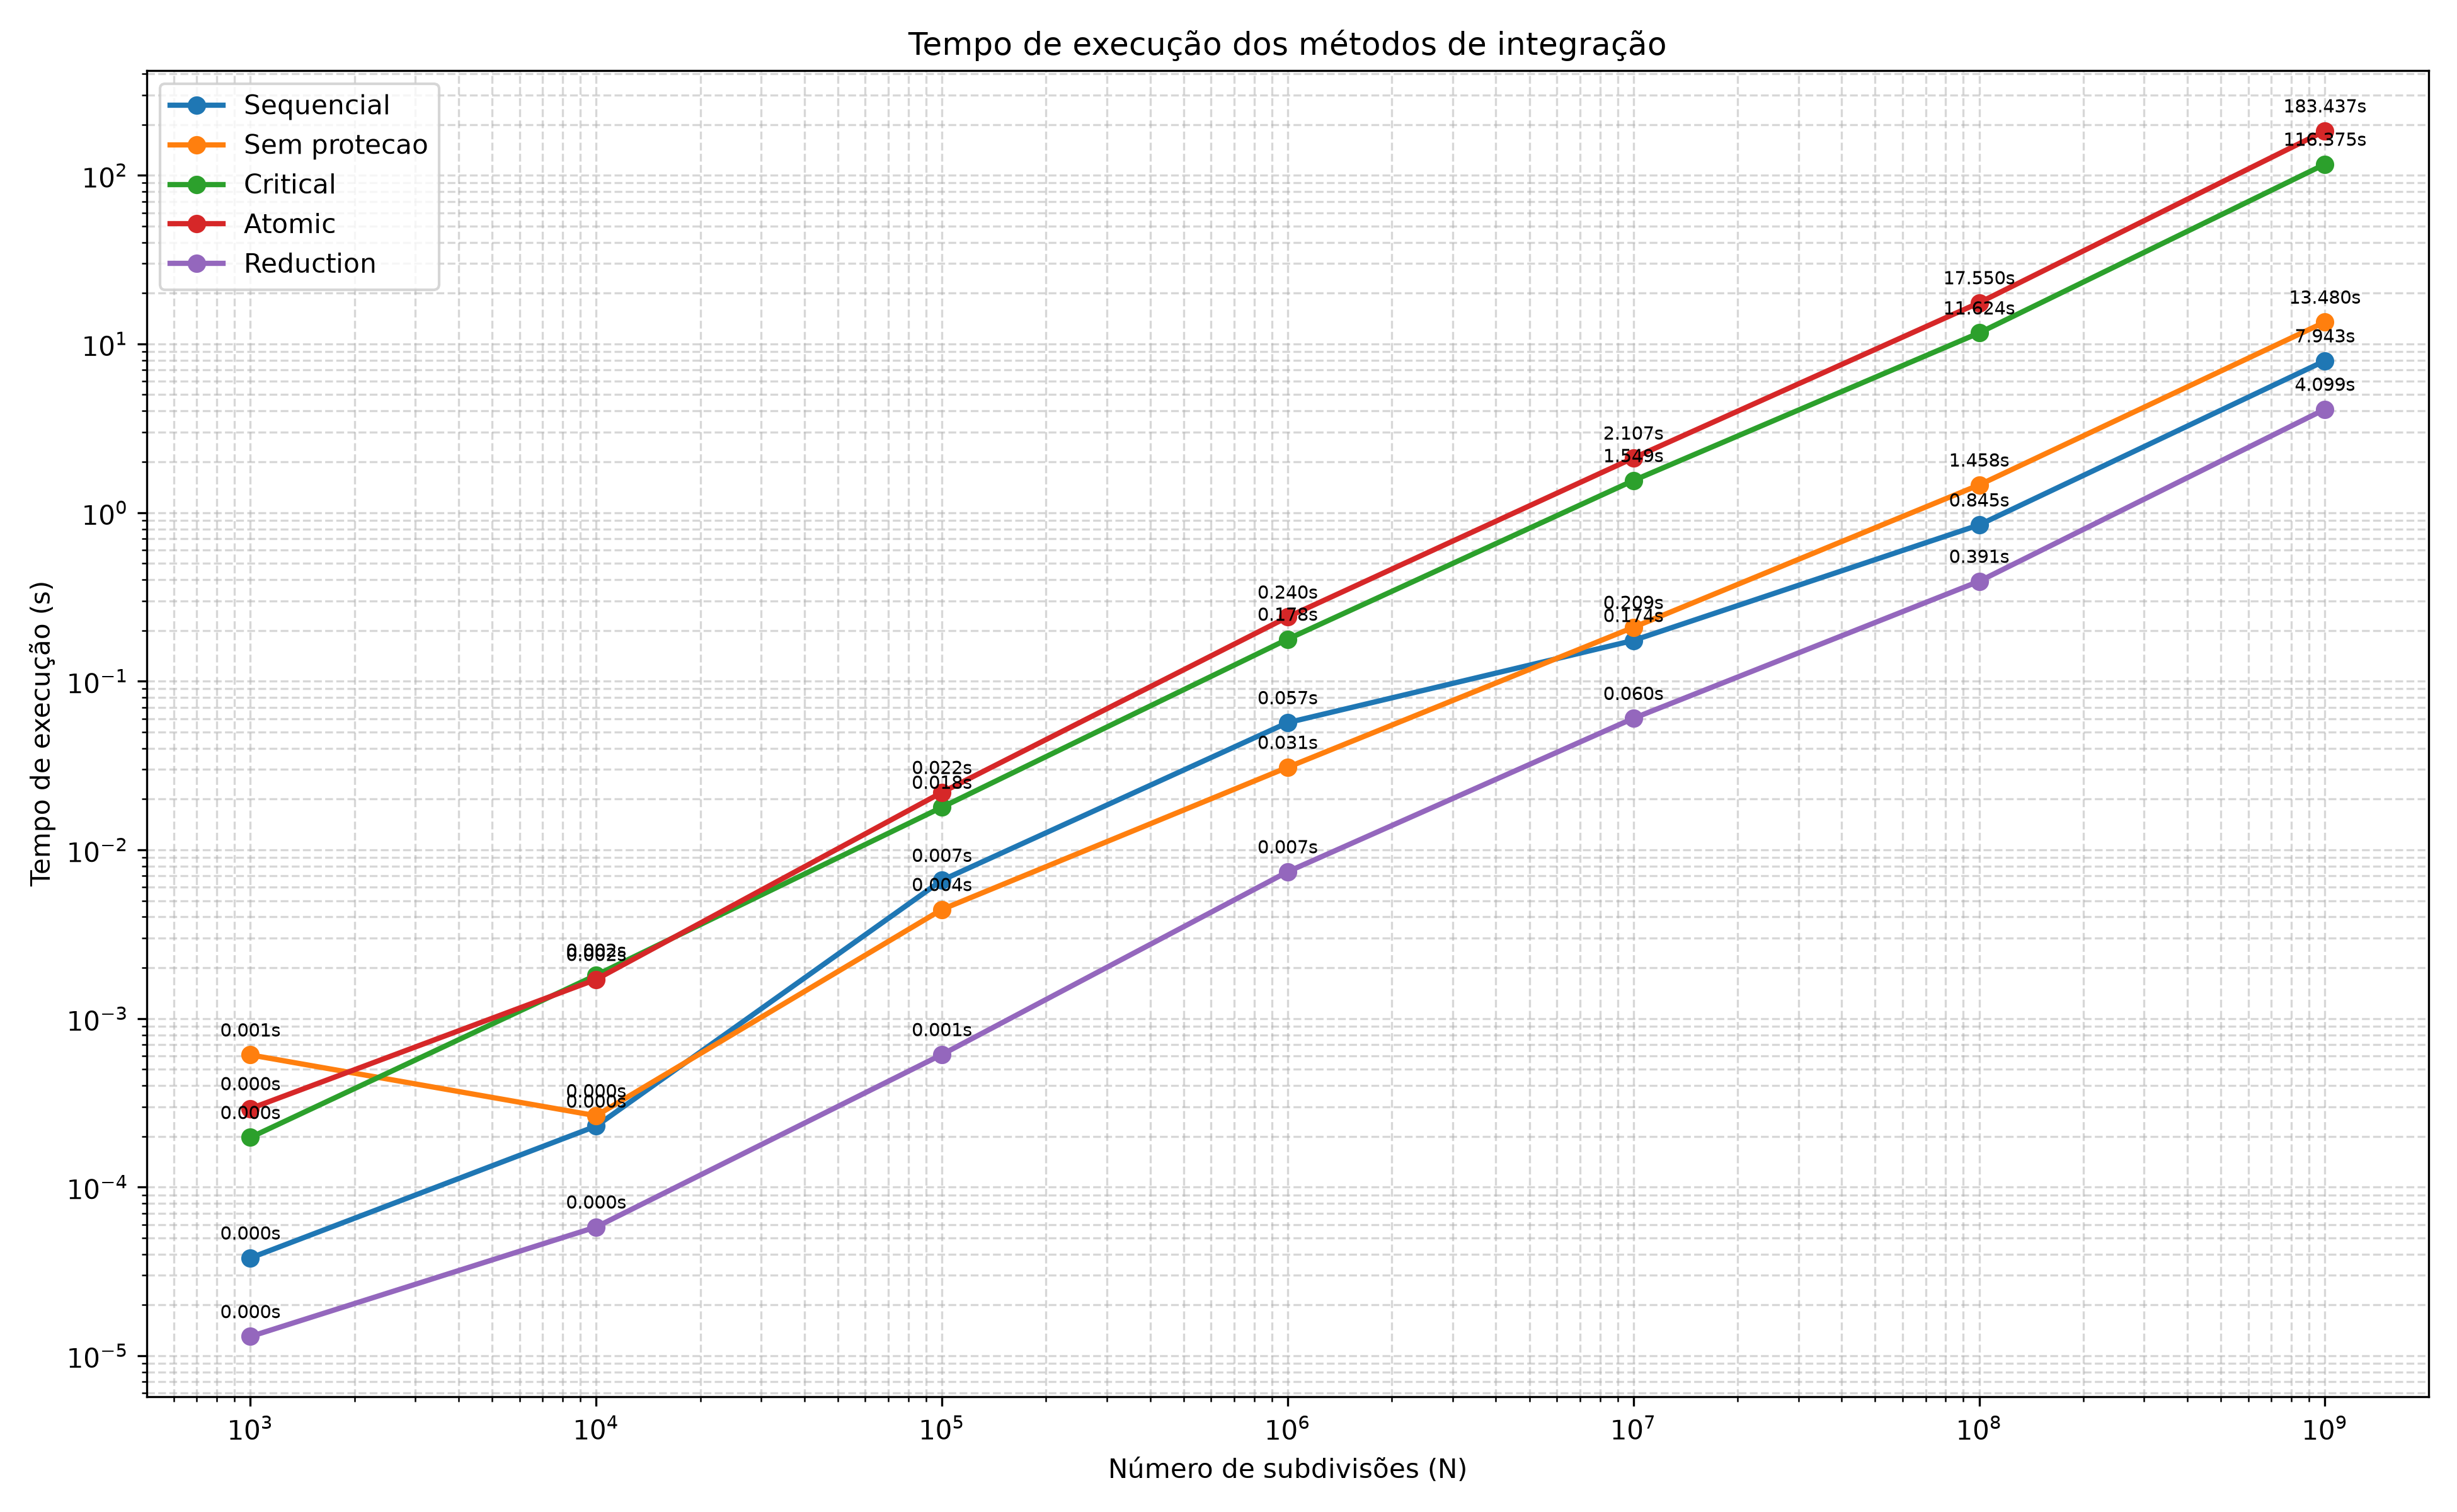
\includegraphics[width=1\textwidth]{Tarefa6/tarefa6tempos.png}
			\end{figure}
			\begin{figure}[H]
				\centering
				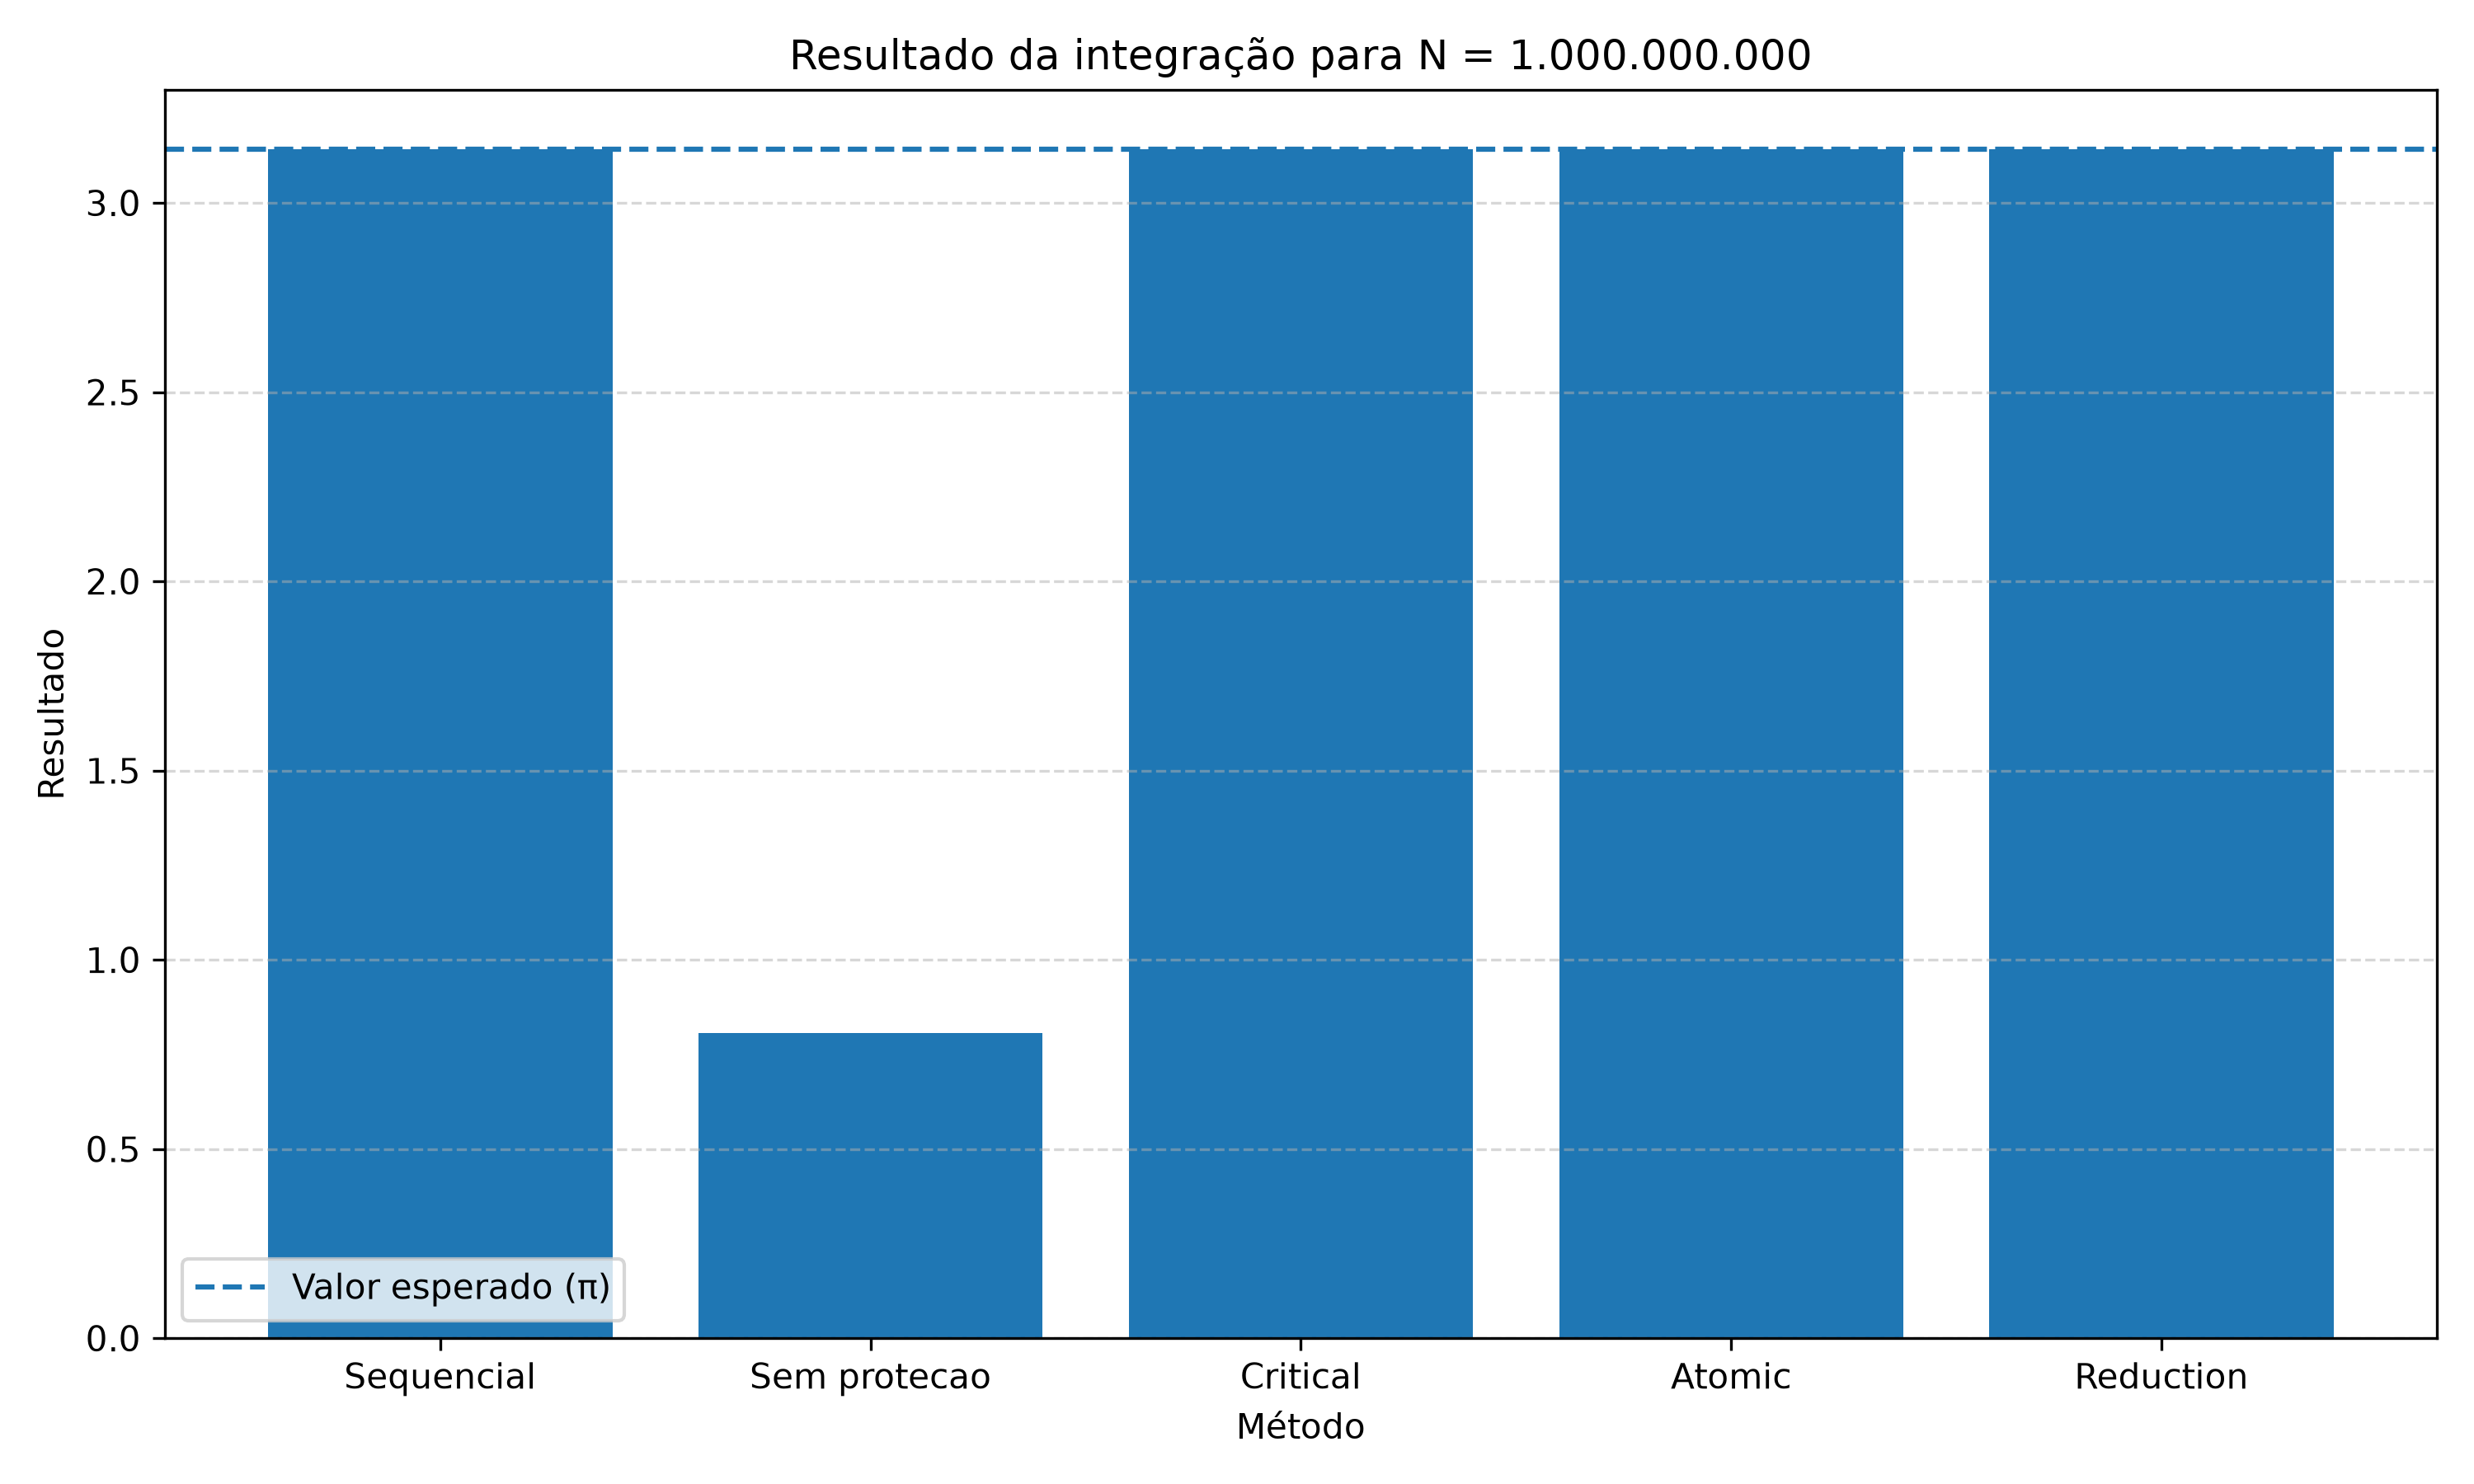
\includegraphics[width=1\textwidth]{Tarefa6/tarefa6barras.png}
			\end{figure}
			\par{Analisando os gráficos, podemos verificar que o único método que obteve um resultado incorreto foi o método sem proteção, devido a um problema de condição de corrida característico da falta de sincronização nesse tipo de implementação.}
			\par{A versão sequencial define uma base para a análise dos resultados das outras implementações. A partir dela podemos verificar que as versões com \texttt{critical} e \texttt{atomic}, apesar de sequenciais, tiveram um tempo maior de execução, pois definem uma área (variável) em que apenas uma thread pode fazer mudanças por vez, o que acaba enfileirando comandos e causando um gargalo que cresce exponencialmente em relação a \texttt{n}, chegando a mais de 100 segundos para \texttt{n = 1000000000}.}
			\par{Já a versão \texttt{reduction} apresenta desempenho significativamente superior, superando tanto as outras versões de paralelismo como também a versão sequencial, já que cada thread mantém uma cópia local de soma e combina os resultados à variável original ao final do processamento, eliminando a necessidade de sincronizar cada iteração.}
			\par{}
		\subsection{\subtTres}
			\begin{lstlisting}[language=c]
#include <stdio.h>
#include <stdlib.h>
#include <math.h>
#include <omp.h>

#define PI_REF 3.14159265358979323846

typedef double (*func_t)(double);

static double f(double x)
{
	return 4.0 / (1.0 + x * x);
}

double trapezio_sequencial(func_t fn, double a, double b, long n)
{
	double h = (b - a) / (double)n;
	double soma = (fn(a) + fn(b)) / 2.0;
	
	for (long i = 1; i < n; i++)
	{
		soma += fn(a + i * h);
	}
	
	return soma * h;
}

double trapezio_paralelo_sem_protecao(func_t fn, double a, double b, long n)
{
	double h = (b - a) / (double)n;
	double soma = (fn(a) + fn(b)) / 2.0;
	
	#pragma omp parallel for
	for (long i = 1; i < n; i++)
	{
		soma += fn(a + i * h);
	}
	
	return soma * h;
}

double trapezio_paralelo_critical(func_t fn, double a, double b, long n)
{
	double h = (b - a) / (double)n;
	double soma = (fn(a) + fn(b)) / 2.0;
	
	#pragma omp parallel for
	for (long i = 1; i < n; i++)
	{
		double parcial = fn(a + i * h);
		
		#pragma omp critical
		{
			soma += parcial;
		}
	}
	
	return soma * h;
}

double trapezio_paralelo_atomic(func_t fn, double a, double b, long n)
{
	double h = (b - a) / (double)n;
	double soma = (fn(a) + fn(b)) / 2.0;
	
	#pragma omp parallel for
	for (long i = 1; i < n; i++)
	{
		double parcial = fn(a + i * h);
		
		#pragma omp atomic
		soma += parcial;
	}
	
	return soma * h;
}

double trapezio_paralelo_reduction(func_t fn, double a, double b, long n)
{
	double h = (b - a) / (double)n;
	double soma = (fn(a) + fn(b)) / 2.0;
	
	#pragma omp parallel for reduction(+:soma)
	for (long i = 1; i < n; i++)
	{
		soma += fn(a + i * h);
	}
	
	return soma * h;
}

typedef double (*trapezio_fn_t)(func_t, double, double, long);

typedef struct
{
	const char *nome;
	double resultado;
	double tempo;
} resultado_t;

static resultado_t executar(
const char *nome,
trapezio_fn_t versao,
func_t fn,
double a,
double b,
long n)
{
	double inicio = omp_get_wtime();
	
	double resultado = versao(fn, a, b, n);
	
	double fim = omp_get_wtime();
	
	double tempo = fim - inicio;
	
	printf(
	"N: %-10ld | Metodo: %-20s | Resultado: %.10f | Tempo: %.6fs\n",
	n,
	nome,
	resultado,
	tempo
	);
	
	return (resultado_t){nome, resultado, tempo};
}

static void exportar_csv(
const char *caminho,
long tamanho_n,
resultado_t *resultados,
int total)
{
	FILE *arquivo = fopen(caminho, "a");
	
	if (!arquivo)
	{
		fprintf(stderr, "Erro ao abrir arquivo CSV: %s\n", caminho);
		return;
	}
	
	for (int i = 0; i < total; i++)
	{
		fprintf(
		arquivo,
		"%ld,%s,%.10f,%.6f\n",
		tamanho_n,
		resultados[i].nome,
		resultados[i].resultado,
		resultados[i].tempo
		);
	}
	
	fclose(arquivo);
}

int main()
{
	double a = 0.0;
	double b = 1.0;
	
	const size_t valores_n[] =
	{
		1000,
		10000,
		100000,
		1000000,
		10000000,
		100000000,
		1000000000
	};
	
	const size_t quantidade_n =
	sizeof(valores_n) / sizeof(valores_n[0]);
	
	int num_threads = omp_get_max_threads();
	
	omp_set_num_threads(num_threads);
	
	const char *csv_path = "resultados.csv";
	
	FILE *arquivo = fopen(csv_path, "w");
	
	if (!arquivo)
	{
		fprintf(stderr, "Erro ao criar arquivo CSV: %s\n", csv_path);
		return EXIT_FAILURE;
	}
	
	fprintf(
	arquivo,
	"tamanho_n,metodo,resultado,tempo\n"
	);
	
	fclose(arquivo);
	
	for (size_t i = 0; i < quantidade_n; i++)
	{
		long n = valores_n[i];
		
		printf("\n============================================\n");
		printf("N = %ld\n", n);
		printf("============================================\n");
		
		resultado_t resultados[5];
		
		resultados[0] = executar(
		"Sequencial",
		trapezio_sequencial,
		f,
		a,
		b,
		n
		);
		
		resultados[1] = executar(
		"Sem protecao",
		trapezio_paralelo_sem_protecao,
		f,
		a,
		b,
		n
		);
		
		resultados[2] = executar(
		"Critical",
		trapezio_paralelo_critical,
		f,
		a,
		b,
		n
		);
		
		resultados[3] = executar(
		"Atomic",
		trapezio_paralelo_atomic,
		f,
		a,
		b,
		n
		);
		
		resultados[4] = executar(
		"Reduction",
		trapezio_paralelo_reduction,
		f,
		a,
		b,
		n
		);
		
		exportar_csv(
		csv_path,
		n,
		resultados,
		5
		);
	}
	
	printf("\nResultados exportados para %s\n", csv_path);
	
	return EXIT_SUCCESS;
}
			\end{lstlisting}
	
	\newpage
		\onehalfspacing
		\section{TAREFA 7}
		\subsection{\subtUm}
		\par{Implementar  diversas versões de um programa que calcule a quantidade de números primos entre 2 e um valor n, utilizando técnicas de paralelização do OpenMP. Comparar o comportamento e resultados e escolher a melhor versão, implementando nela diferentes estratégias de escalonamento. Discutir o resultado observado para cada versão de escalonamento.}
		\subsection{\subtDois}
		\begin{figure}[H]
			\centering
			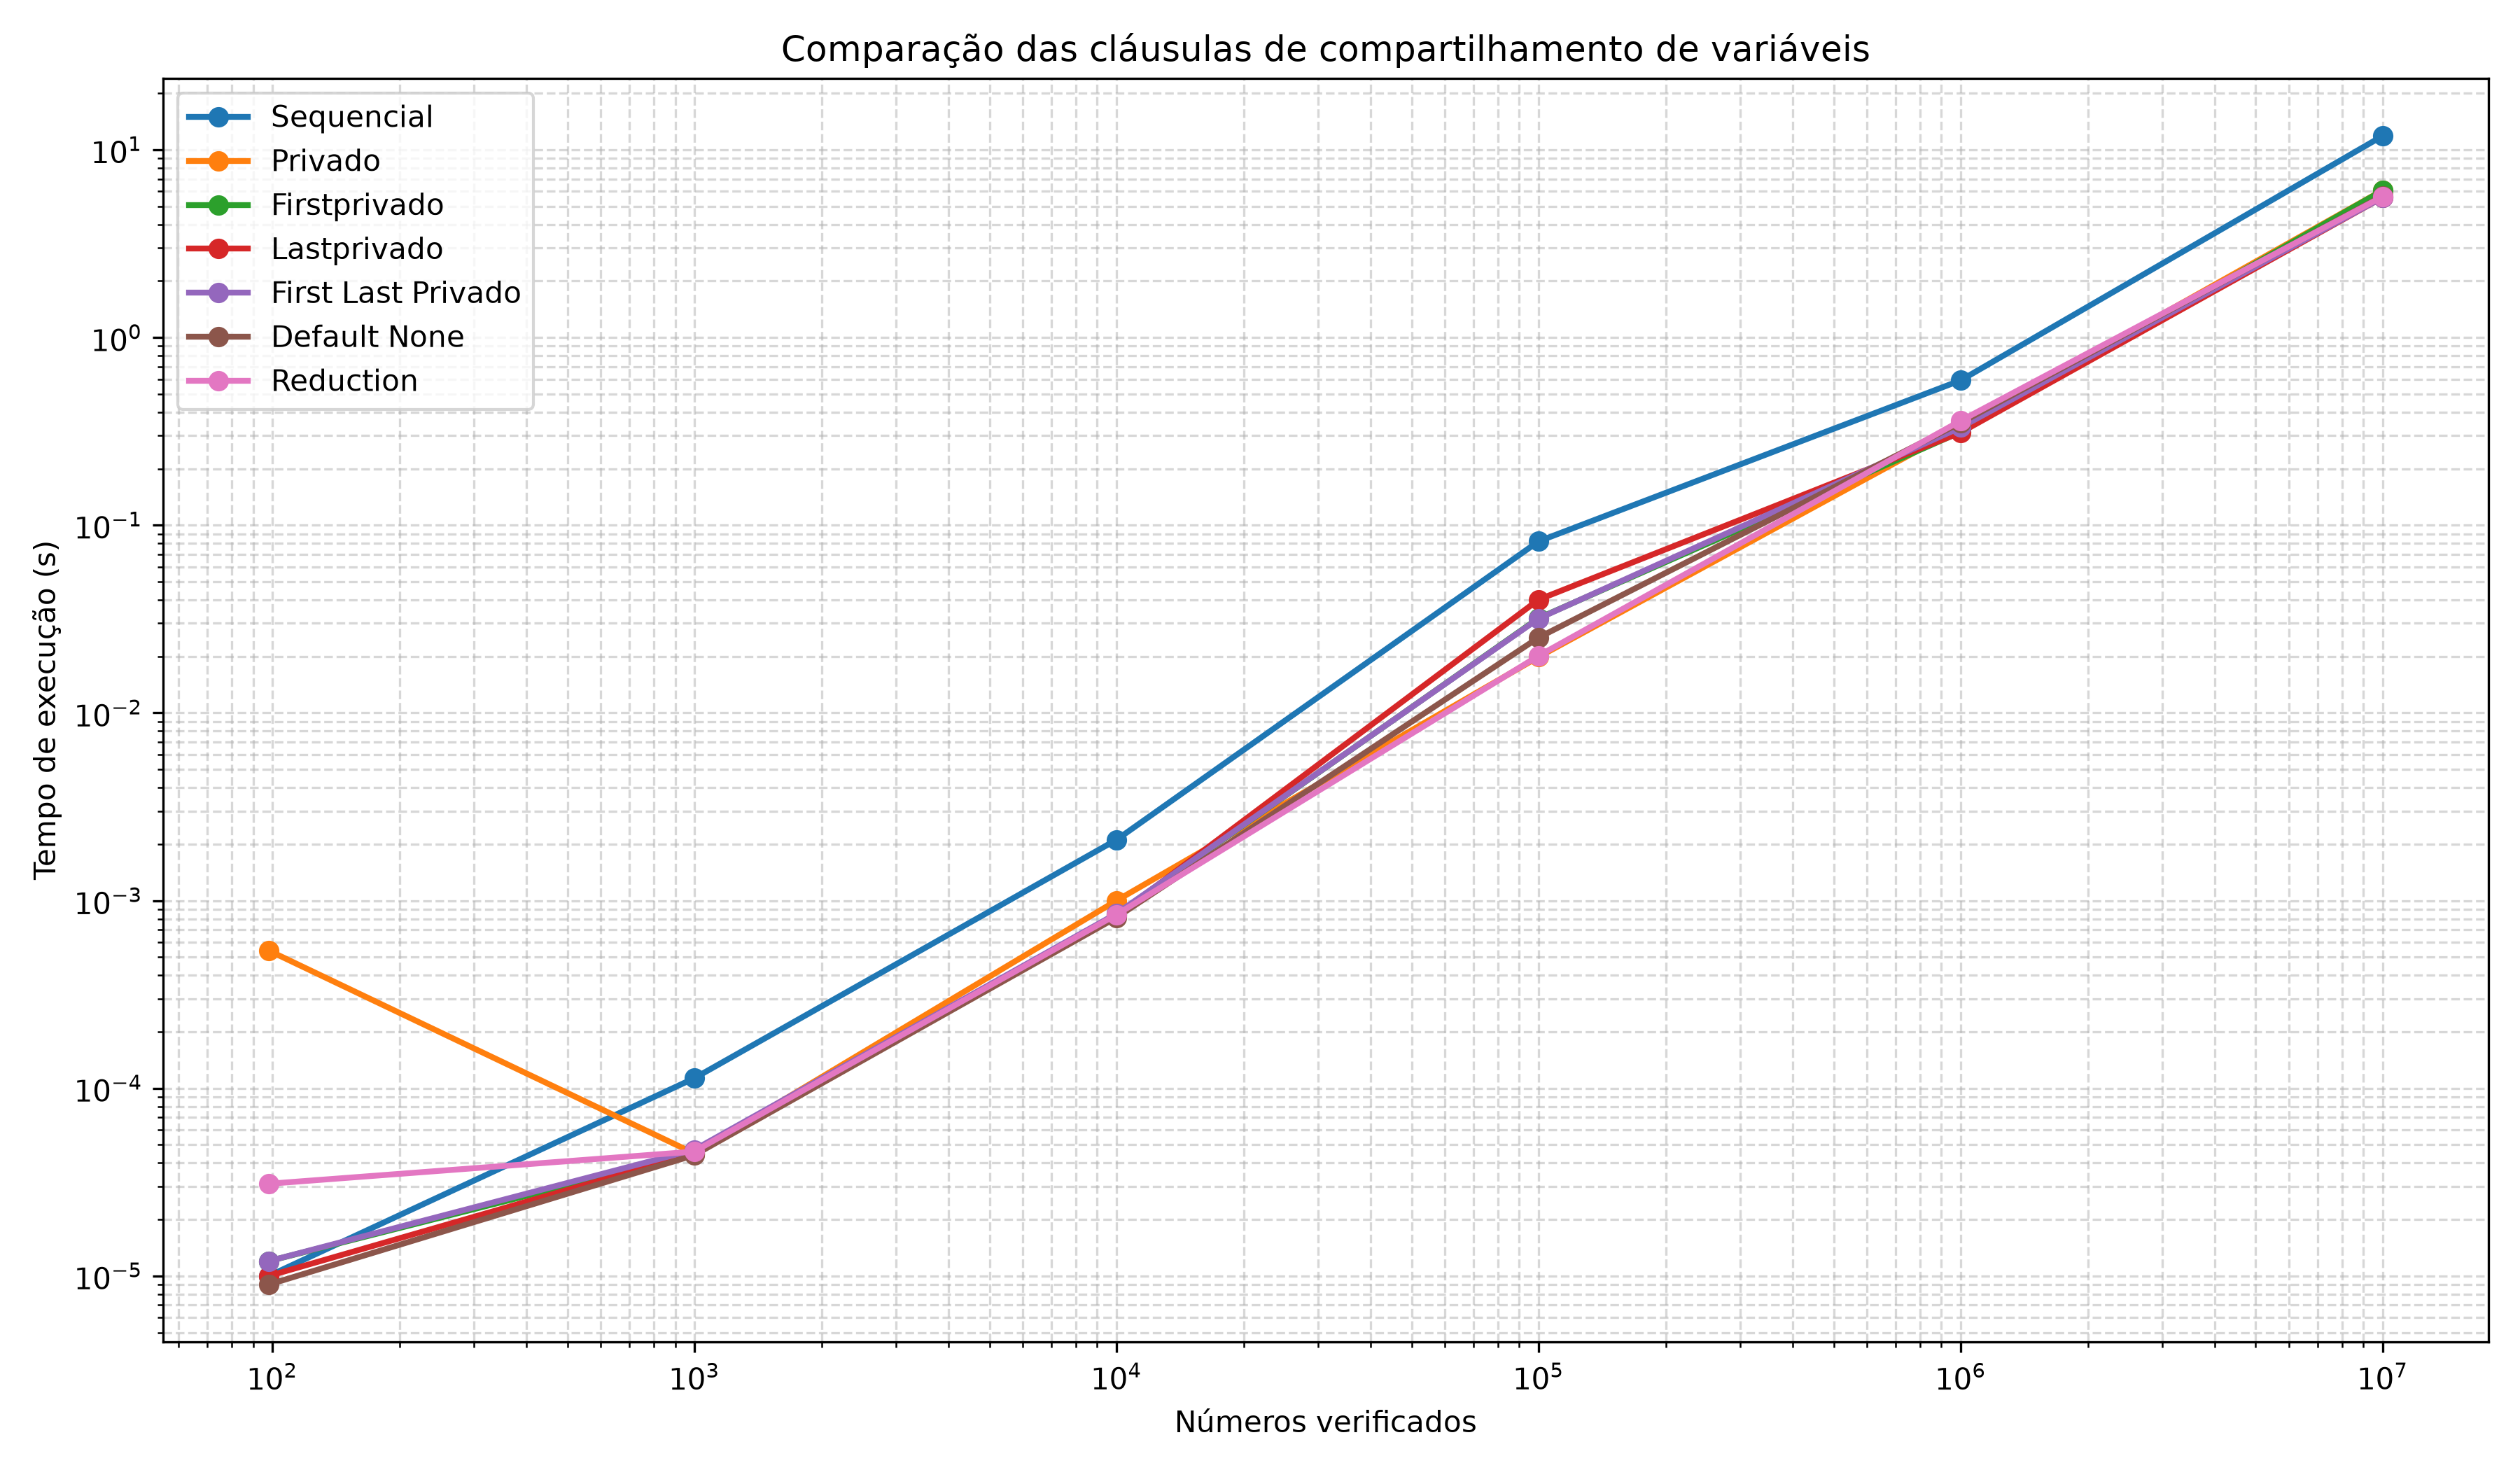
\includegraphics[width=1\textwidth]{Tarefa7/tarefa71.png}
		\end{figure}
		\begin{figure}[H]
			\centering
			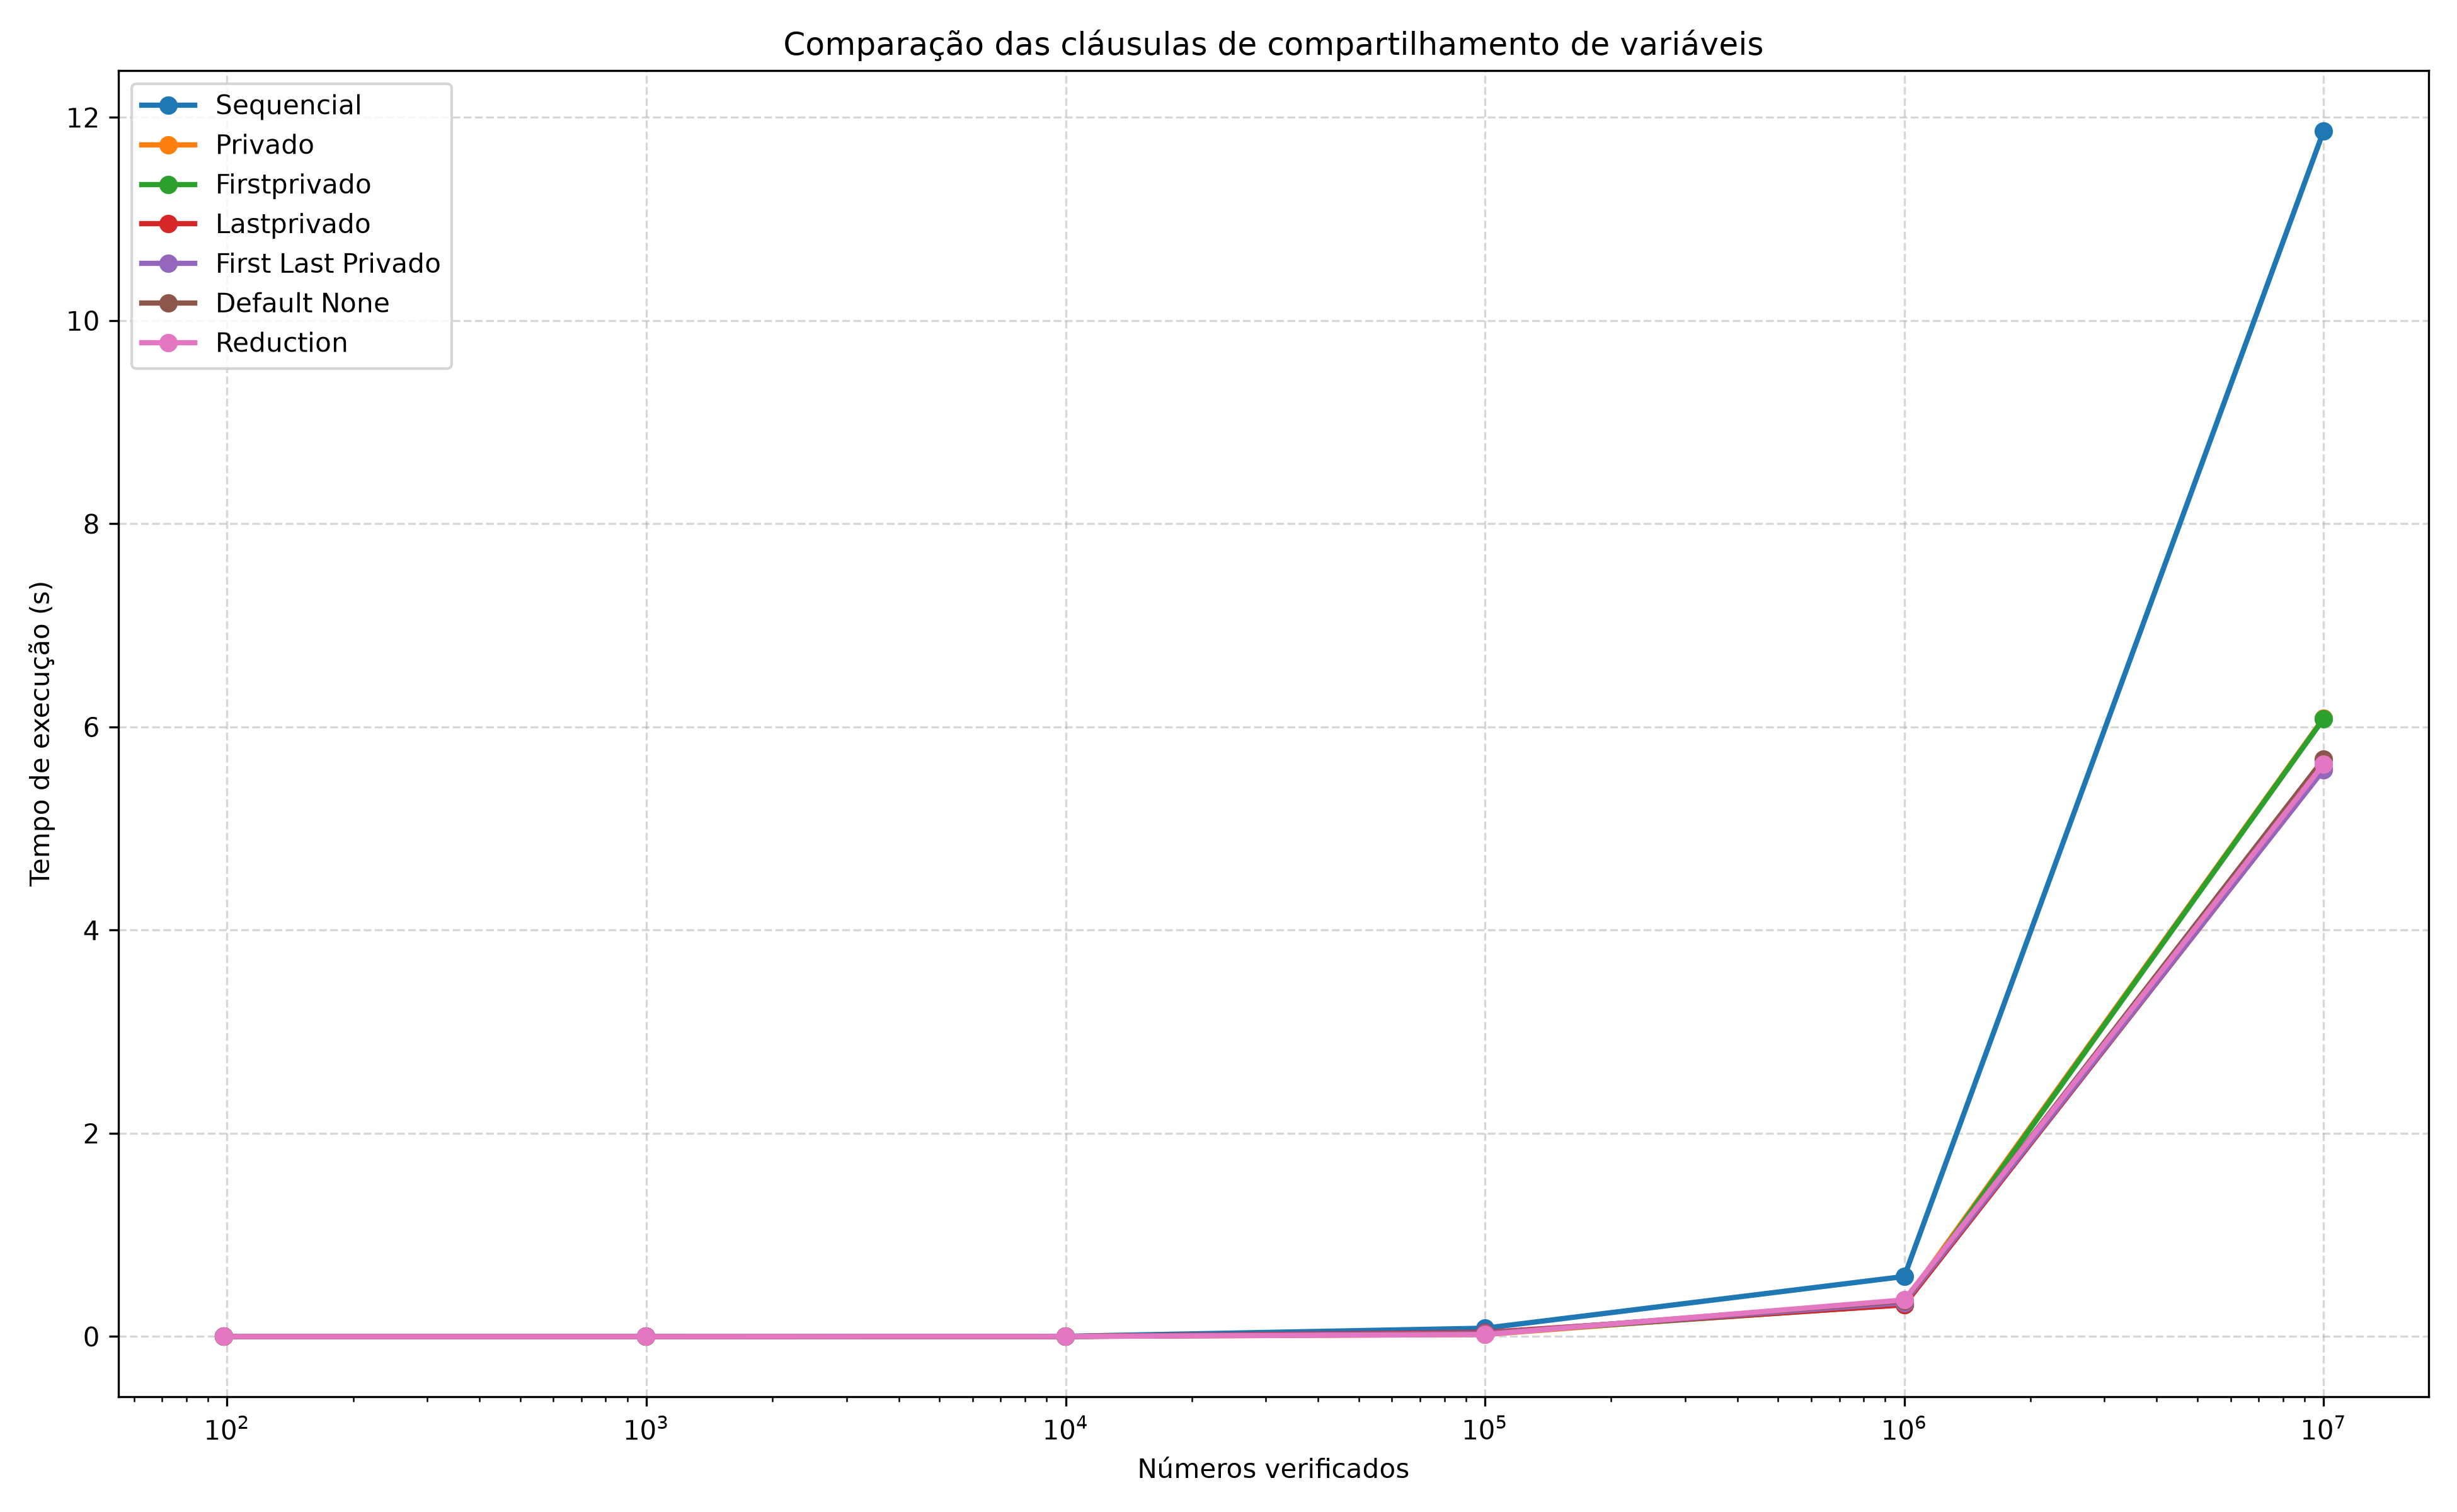
\includegraphics[width=1\textwidth]{Tarefa7/tarefa7versoes.png}
		\end{figure}
		\begin{itemize}
			\item A versão paralela faz a contagem correta, é melhor para valores pequenos devido ao overhead das versões paralelas, mas se torna muito inferior para valores maiores;
			
			\item Com o contador \texttt{private}, cada cópia recebe uma cópia privada da variável \texttt{primos\_encontrados}, portanto a contagem de primos terminou em 0;
			
			\item Com \texttt{firstprivate}, cada thread recebe uma cópia da variável, mas não combina os resultados com a original, terminando em 0 também;
			
			\item Com \texttt{lastprivate}, é copiado para a variável original o valor da variável privada da thread que executou a última iteração do loop;
			
			\item Com \texttt{firstprivate} e \texttt{lastprivate}, cada thread inicia com 0 e, ao terminar, o valor da cópia associada à última iteração é copiado de volta;
			
			\item Com \texttt{reduction}, cada thread tem um contador local que é somado à variável original ao finalizar a contagem, retornando um resultado igual ao da versão sequencial, porém com um tempo de execução muito menor para valores acima de 1000, sendo assim a versão escolhida para o próximo passo.
		\end{itemize}
		\begin{figure}[H]
			\centering
			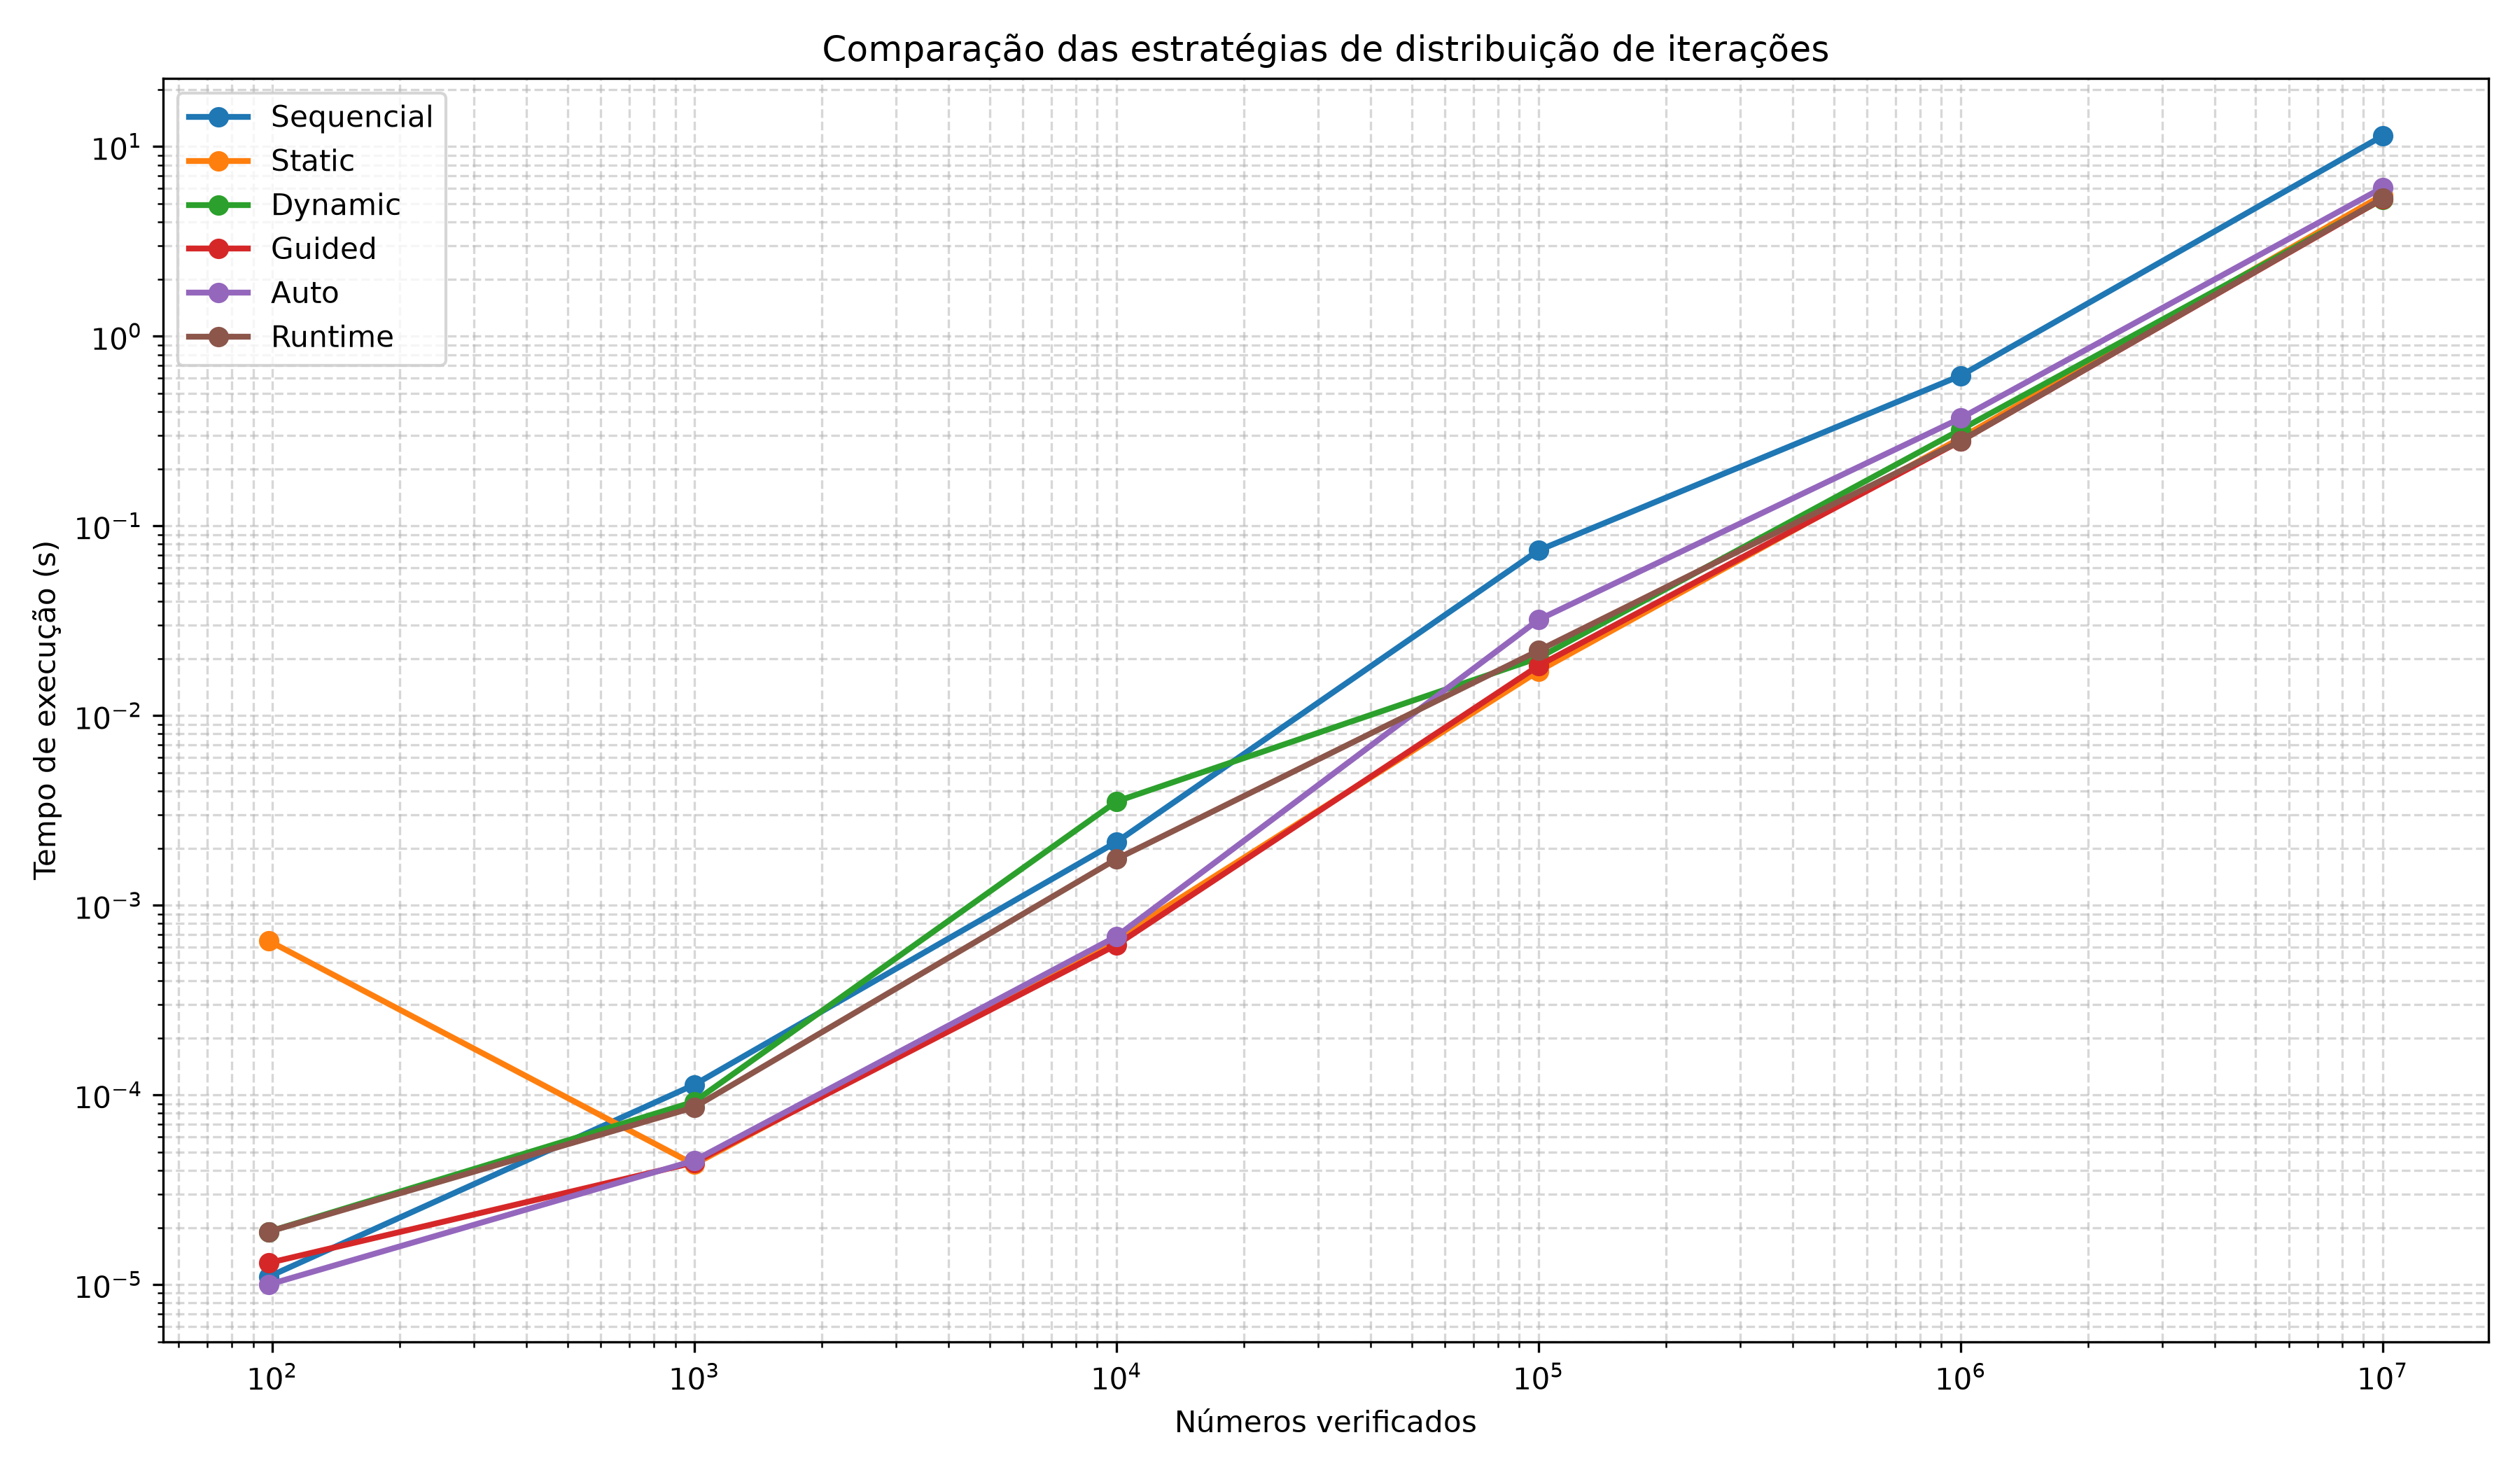
\includegraphics[width=1\textwidth]{Tarefa7/tarefa72.png}
		\end{figure}
		\begin{figure}[H]
			\centering
			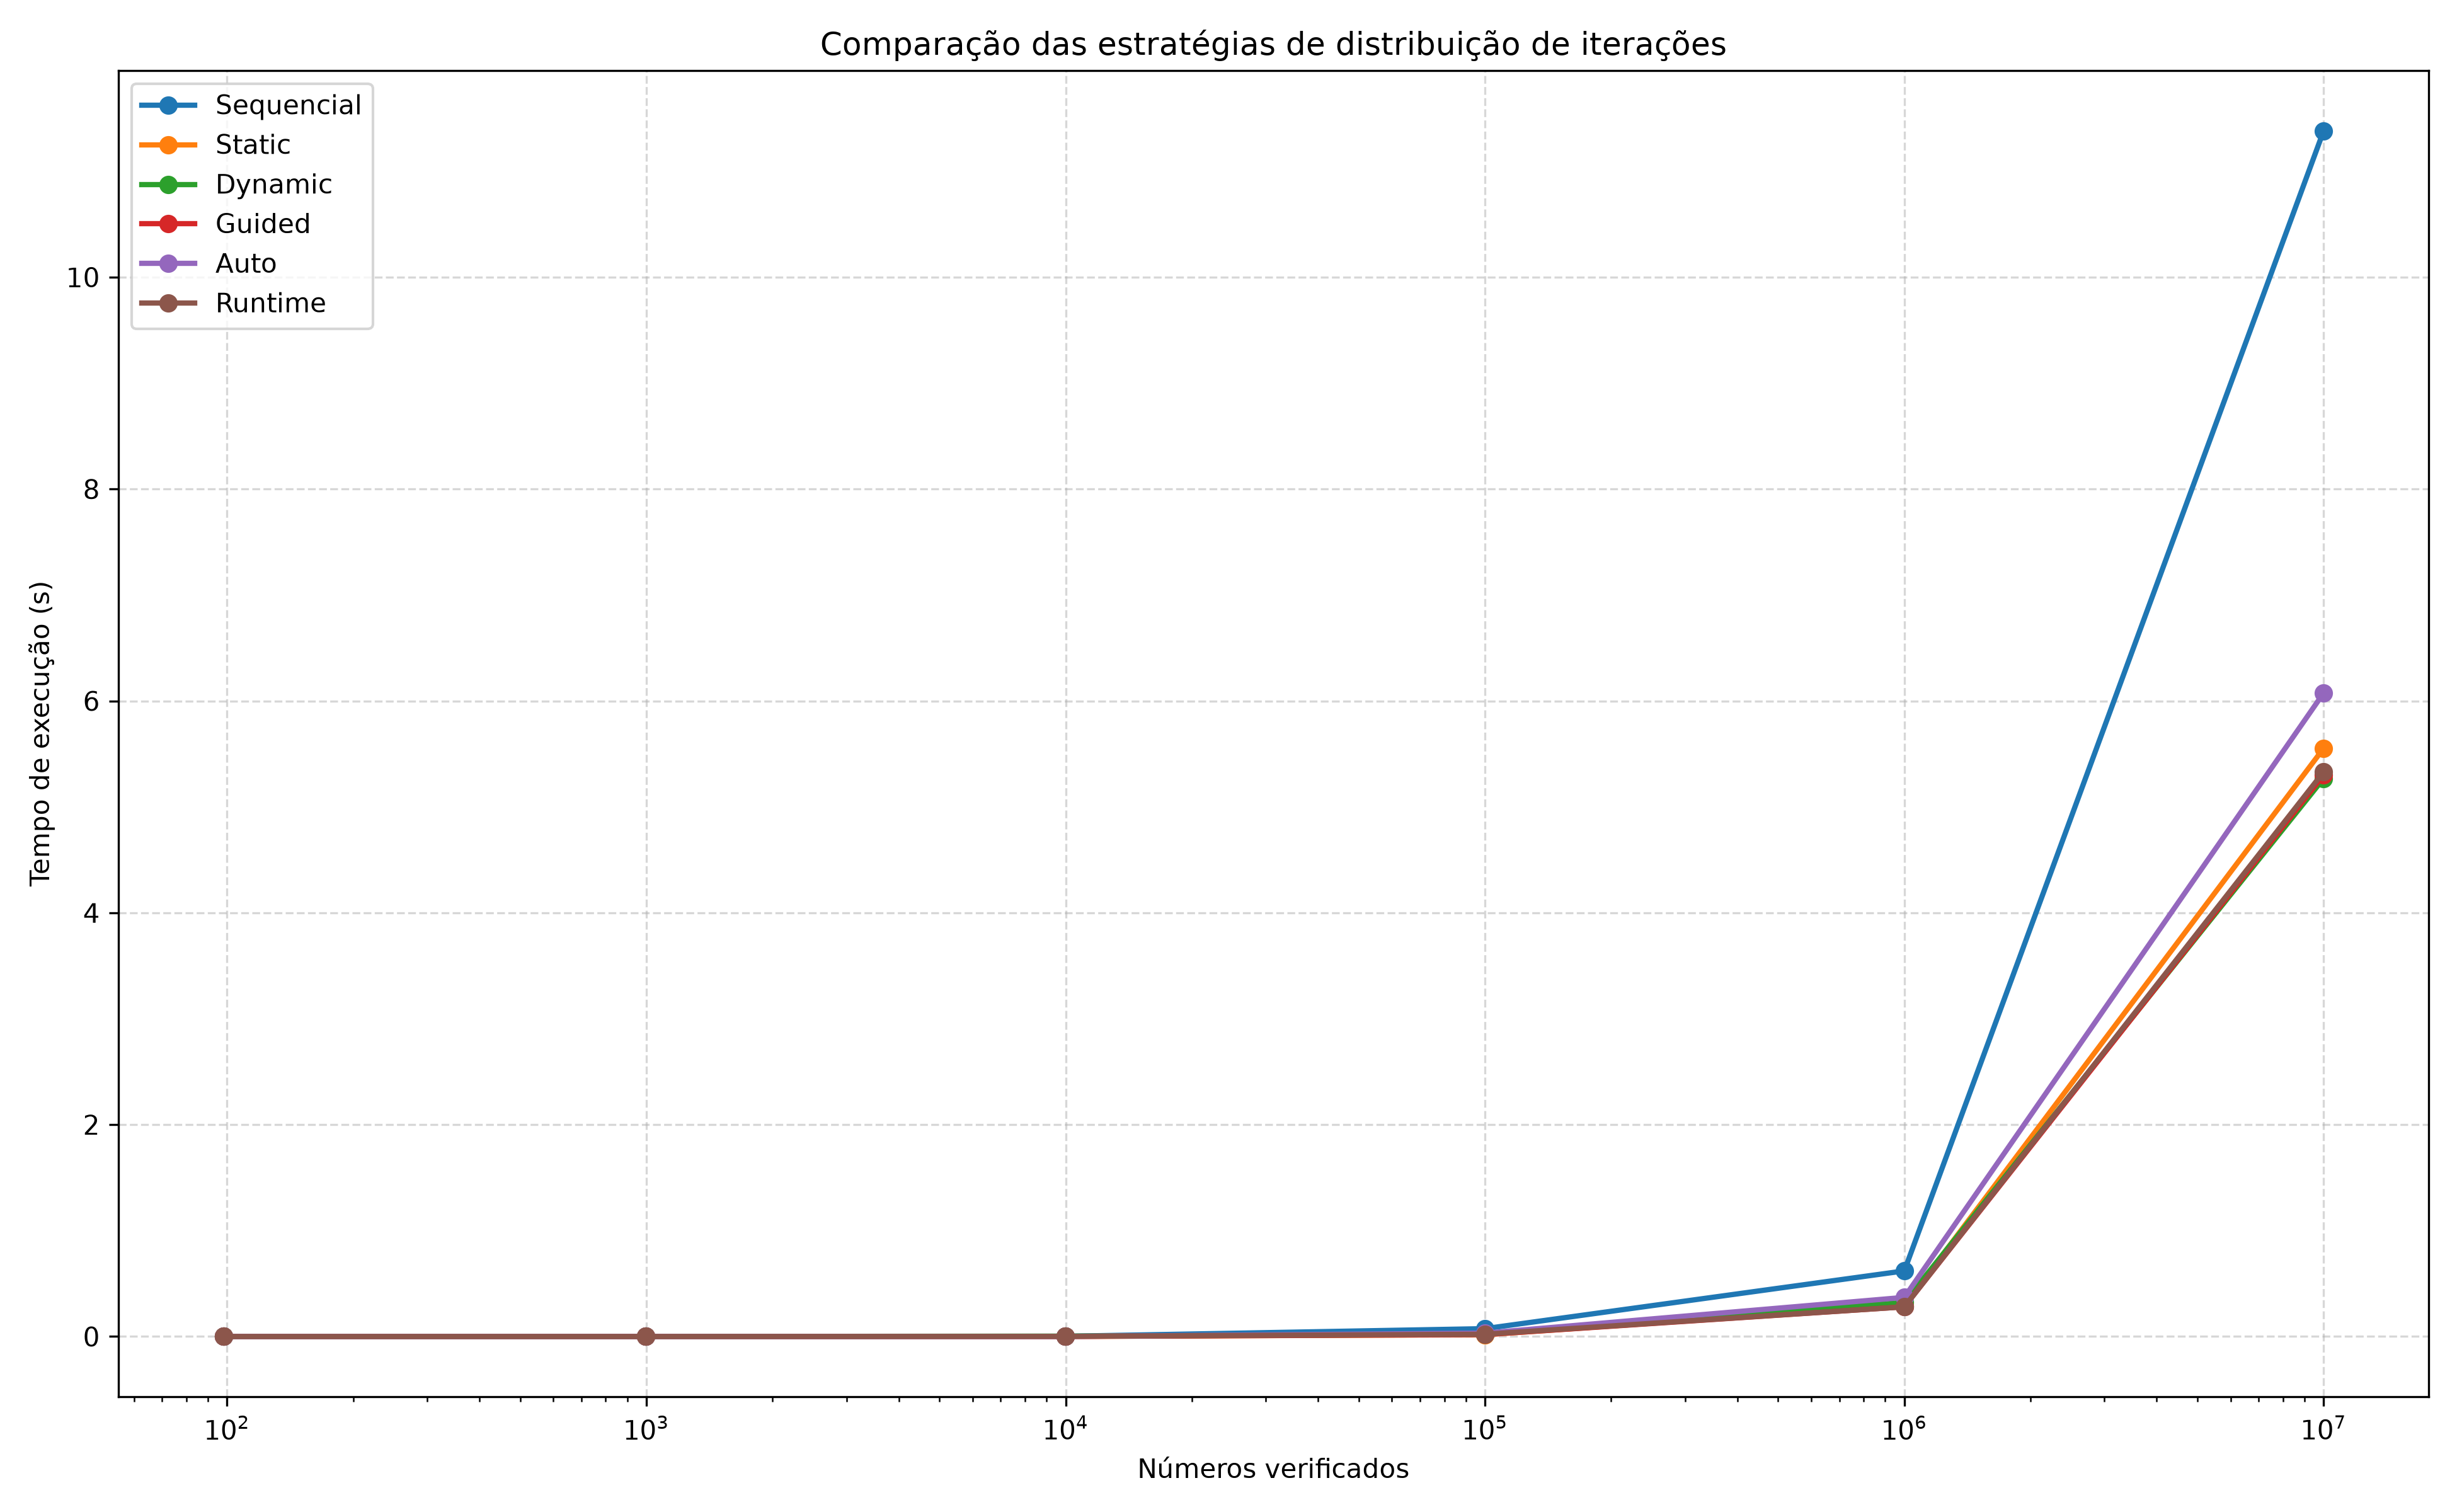
\includegraphics[width=1\textwidth]{Tarefa7/tarefa7esc.png}
		\end{figure}
		\par{Analisando os gráficos dos resultados dos escalonadores, é possível verificar que todos são melhores que a versão sequencial. Comparando entre eles, os resultados indicam que não existe uma diferença significativa entre os escalonadores para conjuntos muito pequenos, pois o overhead do paralelismo representa uma parcela considerável do tempo total.}
		\par{O escalonador \texttt{auto} apresentou os maiores tempos entre as versões paralelas nos conjuntos maiores. O \texttt{auto} permite que o compilador ou a implementação do OpenMP determine a estratégia de distribuição. Como essa decisão é feita automaticamente, seu desempenho depende da implementação utilizada e das características do ambiente de execução, podendo não resultar na estratégia mais eficiente para este problema específico.}
		\par{O \texttt{static} apresenta baixa sobrecarga e comportamento estável, enquanto \texttt{dynamic} e \texttt{guided} podem obter vantagem ao lidar com iterações que apresentam custos muito diferentes. O \texttt{auto} depende da decisão tomada pela implementação do OpenMP e apresentou desempenho inferior nos testes maiores. O \texttt{runtime} apresentou desempenho semelhante ao \texttt{dynamic} e ao \texttt{guided}, além de oferecer a possibilidade de alterar a política de escalonamento sem modificar o código.}
		\subsection{\subtTres}
		\begin{lstlisting}
// main.c
#include <omp.h>
#include <stdbool.h>
#include <stdio.h>

bool isPrimo(int numero) {
	if (numero < 2) {
		return false;
	}
	
	for (int i = 2; i * i <= numero; i++) {
		if (numero % i == 0) {
			return false;
		}
	}
	
	return true;
}

double contarSequencial(int num_inicio, int num_fim) {
	int numeros_verificados = num_fim - num_inicio;
	int primos_encontrados = 0;
	
	double tempo_i = omp_get_wtime();
	
	for (int i = num_inicio + 1; i < num_fim; i++) {
		if (isPrimo(i)) {
			primos_encontrados++;
		}
	}
	
	double tempo_f = omp_get_wtime();
	double tempo_gasto = tempo_f - tempo_i;
	
	printf("[SEQ] | # Verificados: %d | Primos: %d | Tempo: %f\n",
	numeros_verificados, primos_encontrados, tempo_gasto);
	
	return tempo_gasto;
}

double contarParaleloPrivado(int num_inicio, int num_fim) {
	int numeros_verificados = num_fim - num_inicio;
	int primos_encontrados = 0;
	
	double tempo_i = omp_get_wtime();
	
	#pragma omp parallel for private(primos_encontrados)
	for (int i = num_inicio + 1; i < num_fim; i++) {
		if (isPrimo(i)) {
			primos_encontrados++;
		}
	}
	
	double tempo_f = omp_get_wtime();
	double tempo_gasto = tempo_f - tempo_i;
	
	printf("[PRIVATE] | # Verificados: %d | Primos: %d | Tempo: %f\n",
	numeros_verificados, primos_encontrados, tempo_gasto);
	
	return tempo_gasto;
}

double contarParaleloFirstPrivado(int num_inicio, int num_fim) {
	int numeros_verificados = num_fim - num_inicio;
	int primos_encontrados = 0;
	
	double tempo_i = omp_get_wtime();
	
	#pragma omp parallel for firstprivate(primos_encontrados)
	for (int i = num_inicio + 1; i < num_fim; i++) {
		if (isPrimo(i)) {
			primos_encontrados++;
		}
	}
	
	double tempo_f = omp_get_wtime();
	double tempo_gasto = tempo_f - tempo_i;
	
	printf("[FIRSTPRIVATE] | # Verificados: %d | Primos: %d | Tempo: %f\n",
	numeros_verificados, primos_encontrados, tempo_gasto);
	
	return tempo_gasto;
}

double contarParaleloLastPrivado(int num_inicio, int num_fim) {
	int numeros_verificados = num_fim - num_inicio;
	int primos_encontrados = 0;
	
	double tempo_i = omp_get_wtime();
	
	#pragma omp parallel for lastprivate(primos_encontrados)
	for (int i = num_inicio + 1; i < num_fim; i++) {
		if (isPrimo(i)) {
			primos_encontrados++;
		}
	}
	
	double tempo_f = omp_get_wtime();
	double tempo_gasto = tempo_f - tempo_i;
	
	printf("[LASTPRIVATE] | # Verificados: %d | Primos: %d | Tempo: %f\n",
	numeros_verificados, primos_encontrados, tempo_gasto);
	
	return tempo_gasto;
}

double contarParaleloFirstLastPrivado(int num_inicio, int num_fim) {
	int numeros_verificados = num_fim - num_inicio;
	int primos_encontrados = 0;
	
	double tempo_i = omp_get_wtime();
	
	#pragma omp parallel for firstprivate(primos_encontrados) lastprivate(primos_encontrados)
	for (int i = num_inicio + 1; i < num_fim; i++) {
		if (isPrimo(i)) {
			primos_encontrados++;
		}
	}
	
	double tempo_f = omp_get_wtime();
	double tempo_gasto = tempo_f - tempo_i;
	
	printf("[FIRST+LASTPRIVATE] | # Verificados: %d | Primos: %d | Tempo: %f\n",
	numeros_verificados, primos_encontrados, tempo_gasto);
	
	return tempo_gasto;
}

double contarParaleloDefaultNone(int num_inicio, int num_fim) {
	int numeros_verificados = num_fim - num_inicio;
	int primos_encontrados = 0;
	
	double tempo_i = omp_get_wtime();
	
	#pragma omp parallel for default(none) shared(num_inicio, num_fim) private(primos_encontrados)
	for (int i = num_inicio + 1; i < num_fim; i++) {
		if (isPrimo(i)) {
			primos_encontrados++;
		}
	}
	
	double tempo_f = omp_get_wtime();
	double tempo_gasto = tempo_f - tempo_i;
	
	printf("[DEFAULT(NONE)] | # Verificados: %d | Primos: %d | Tempo: %f\n",
	numeros_verificados, primos_encontrados, tempo_gasto);
	
	return tempo_gasto;
}

double contarParaleloReduction(int num_inicio, int num_fim) {
	int numeros_verificados = num_fim - num_inicio;
	int primos_encontrados = 0;
	
	double tempo_i = omp_get_wtime();
	
	#pragma omp parallel for reduction(+ : primos_encontrados)
	for (int i = num_inicio + 1; i < num_fim; i++) {
		if (isPrimo(i)) {
			primos_encontrados++;
		}
	}
	
	double tempo_f = omp_get_wtime();
	double tempo_gasto = tempo_f - tempo_i;
	
	printf("[REDUCTION] | # Verificados: %d | Primos: %d | Tempo: %f\n",
	numeros_verificados, primos_encontrados, tempo_gasto);
	
	return tempo_gasto;
}

int main() {
	int inicio = 2;
	
	const size_t iteracoes[] = {100, 1000, 10000, 100000, 1000000, 10000000};
	
	const size_t quantidade = sizeof(iteracoes) / sizeof(iteracoes[0]);
	
	FILE *arquivo_saida = fopen("resultados7.csv", "w");
	
	if (arquivo_saida == NULL) {
		printf("Erro ao abrir o arquivo CSV.\n");
		return 1;
	}
	
	fprintf(arquivo_saida,
	"numeros_verificados,tempo_sequencial,tempo_privado,"
	"tempo_firstprivado,tempo_lastprivado,"
	"tempo_first_last_privado,tempo_default_none,tempo_reduction\n");
	
	for (size_t i = 0; i < quantidade; i++) {
		int fim = iteracoes[i];
		
		printf("\n====== BUSCANDO PRIMOS ATÉ %d ======\n", fim);
		
		double tempo_sequencial = contarSequencial(inicio, fim);
		double tempo_privado = contarParaleloPrivado(inicio, fim);
		double tempo_firstprivado = contarParaleloFirstPrivado(inicio, fim);
		double tempo_lastprivado = contarParaleloLastPrivado(inicio, fim);
		double tempo_first_last_privado =
		contarParaleloFirstLastPrivado(inicio, fim);
		double tempo_default_none = contarParaleloDefaultNone(inicio, fim);
		double tempo_reduction = contarParaleloReduction(inicio, fim);
		
		fprintf(arquivo_saida,
		"%d,%f,%f,%f,%f,%f,%f,%f\n",
		fim - inicio,
		tempo_sequencial,
		tempo_privado,
		tempo_firstprivado,
		tempo_lastprivado,
		tempo_first_last_privado,
		tempo_default_none,
		tempo_reduction);
	}
	
	fclose(arquivo_saida);
	
	printf("\nResultados salvos em resultados7.csv\n");
	
	return 0;
}
		\end{lstlisting}
		
		\begin{lstlisting}
#include <omp.h>
#include <stdbool.h>
#include <stdio.h>

bool isPrimo(int numero) {
	if (numero < 2) {
		return false;
	}
	
	for (int i = 2; i * i <= numero; i++) {
		if (numero % i == 0) {
			return false;
		}
	}
	
	return true;
}

// sequencial é usado aqui só como parâmetro, pra saber se todas vão contar coretamente
double contarSequencial(int num_inicio, int num_fim) {
	int numeros_verificados = num_fim - num_inicio;
	int primos_encontrados = 0;
	
	double tempo_i = omp_get_wtime();
	
	for (int i = num_inicio + 1; i < num_fim; i++) {
		if (isPrimo(i)) {
			primos_encontrados++;
		}
	}
	
	double tempo_f = omp_get_wtime();
	double tempo_gasto = tempo_f - tempo_i;
	
	printf("[SEQ] | # Verificados: %d | Primos: %d | Tempo: %f\n",
	numeros_verificados, primos_encontrados, tempo_gasto);
	
	return tempo_gasto;
}

double contarParaleloStatic(int num_inicio, int num_fim) {
	int numeros_verificados = num_fim - num_inicio;
	int primos_encontrados = 0;
	
	double tempo_i = omp_get_wtime();
	
	#pragma omp parallel for schedule(static) reduction(+ : primos_encontrados)
	for (int i = num_inicio + 1; i < num_fim; i++) {
		if (isPrimo(i)) {
			primos_encontrados++;
		}
	}
	
	double tempo_f = omp_get_wtime();
	double tempo_gasto = tempo_f - tempo_i;
	
	printf("[STATIC] | # Verificados: %d | Primos: %d | Tempo: %f\n",
	numeros_verificados, primos_encontrados, tempo_gasto);
	
	return tempo_gasto;
}

double contarParaleloDynamic(int num_inicio, int num_fim) {
	int numeros_verificados = num_fim - num_inicio;
	int primos_encontrados = 0;
	
	double tempo_i = omp_get_wtime();
	
	#pragma omp parallel for schedule(dynamic) reduction(+ : primos_encontrados)
	for (int i = num_inicio + 1; i < num_fim; i++) {
		if (isPrimo(i)) {
			primos_encontrados++;
		}
	}
	
	double tempo_f = omp_get_wtime();
	double tempo_gasto = tempo_f - tempo_i;
	
	printf("[DYNAMIC] | # Verificados: %d | Primos: %d | Tempo: %f\n",
	numeros_verificados, primos_encontrados, tempo_gasto);
	
	return tempo_gasto;
}

double contarParaleloGuided(int num_inicio, int num_fim) {
	int numeros_verificados = num_fim - num_inicio;
	int primos_encontrados = 0;
	
	double tempo_i = omp_get_wtime();
	
	#pragma omp parallel for schedule(guided) reduction(+ : primos_encontrados)
	for (int i = num_inicio + 1; i < num_fim; i++) {
		if (isPrimo(i)) {
			primos_encontrados++;
		}
	}
	
	double tempo_f = omp_get_wtime();
	double tempo_gasto = tempo_f - tempo_i;
	
	printf("[GUIDED] | # Verificados: %d | Primos: %d | Tempo: %f\n",
	numeros_verificados, primos_encontrados, tempo_gasto);
	
	return tempo_gasto;
}

double contarParaleloAuto(int num_inicio, int num_fim) {
	int numeros_verificados = num_fim - num_inicio;
	int primos_encontrados = 0;
	
	double tempo_i = omp_get_wtime();
	
	#pragma omp parallel for schedule(auto) reduction(+ : primos_encontrados)
	for (int i = num_inicio + 1; i < num_fim; i++) {
		if (isPrimo(i)) {
			primos_encontrados++;
		}
	}
	
	double tempo_f = omp_get_wtime();
	double tempo_gasto = tempo_f - tempo_i;
	
	printf("[AUTO] | # Verificados: %d | Primos: %d | Tempo: %f\n",
	numeros_verificados, primos_encontrados, tempo_gasto);
	
	return tempo_gasto;
}

double contarParaleloRuntime(int num_inicio, int num_fim) {
	int numeros_verificados = num_fim - num_inicio;
	int primos_encontrados = 0;
	
	double tempo_i = omp_get_wtime();
	
	#pragma omp parallel for schedule(runtime) reduction(+ : primos_encontrados)
	for (int i = num_inicio + 1; i < num_fim; i++) {
		if (isPrimo(i)) {
			primos_encontrados++;
		}
	}
	
	double tempo_f = omp_get_wtime();
	double tempo_gasto = tempo_f - tempo_i;
	
	printf("[RUNTIME] | # Verificados: %d | Primos: %d | Tempo: %f\n",
	numeros_verificados, primos_encontrados, tempo_gasto);
	
	return tempo_gasto;
}

int main() {
	int inicio = 2;
	
	const size_t iteracoes[] = {100, 1000, 10000, 100000, 1000000, 10000000};
	
	const size_t quantidade = sizeof(iteracoes) / sizeof(iteracoes[0]);
	
	FILE *arquivo_saida = fopen("resultados7esc.csv", "w");
	
	if (arquivo_saida == NULL) {
		printf("Erro ao abrir o arquivo CSV.\n");
		return 1;
	}
	
	fprintf(arquivo_saida, "numeros_verificados,"
	"tempo_sequencial,"
	"tempo_static,"
	"tempo_dynamic,"
	"tempo_guided,"
	"tempo_auto,"
	"tempo_runtime\n");
	
	for (size_t i = 0; i < quantidade; i++) {
		int fim = iteracoes[i];
		
		printf("\n====== BUSCANDO PRIMOS ATÉ %d ======\n", fim);
		
		double tempo_sequencial = contarSequencial(inicio, fim);
		
		double tempo_static = contarParaleloStatic(inicio, fim);
		
		double tempo_dynamic = contarParaleloDynamic(inicio, fim);
		
		double tempo_guided = contarParaleloGuided(inicio, fim);
		
		double tempo_auto = contarParaleloAuto(inicio, fim);
		
		double tempo_runtime = contarParaleloRuntime(inicio, fim);
		
		fprintf(arquivo_saida, "%d,%f,%f,%f,%f,%f,%f\n", fim - inicio,
		tempo_sequencial, tempo_static, tempo_dynamic, tempo_guided,
		tempo_auto, tempo_runtime);
	}
	
	fclose(arquivo_saida);
	
	printf("\nResultados salvos em resultados7esc.csv\n");
	
	return 0;
}
		\end{lstlisting}

	\newpage
		\onehalfspacing
		\section{TAREFA 8}
		\subsection{\subtUm}
		\par{Implementar um código com OpenMP que inicializa um vetor que representa uma função qualquer. Calcular a integral desse vetor utilizando o método do trapézio e o vetor que representa a derivada do vetor original. Utilizar diretiva \texttt{sections}.}
		\subsection{\subtDois}
			\par{O paralelismo de tarefas no código é feito a partir do uso das diretivas \texttt{\#pragma omp parallel sections} e \texttt{\#pragma omp section}, que dividem a execução principal entre duas tarefas independentes e concorrentes: o cálculo da integral e o cálculo da derivada.}
			\par{O paralelismo de dados se dá pelas diretivas \texttt{\#pragma omp parallel} e \texttt{\#pragma omp for}, dentro do escopo de cada iteração, que é dividida em blocos para que cada thread processe individualmente. Além disso, a diretiva \texttt{reduction} utilizada também divide os dados usados por threads para somar à variável original posteriormente.}
			\par{O aninhamento das regiões paralelas é feito a partir das funções do OpenMP \texttt{omp\_set\_nested(1)}, que habilita essa funcionalidade de aninhamento, e \texttt{omp\_set\_max\_active\_levels(2)}, que define o nível máximo de profundidade como 2.}
			\par{A garantia de execução de determinadas ações por uma única thread é dada pela diretiva \texttt{\#pragma omp single}, que faz com que apenas a primeira thread interna a atingir o bloco executa as instruções, enquanto as demais threads ignoram a execução do bloco.}
			\par{Os mecanismos de sincronização utilizados foram: barreiras implícitas, que garantem que certas fases do programa terminaram antes de avançar a execução; Diretiva \texttt{reduction}, que permite a sincronização de threads no acesso e gerenciamento do valor de determinado local de dados, impedindo locks e regiões críticas.}
		\subsection{\subtTres}
		\begin{lstlisting}
#include <stdio.h>
#include <stdlib.h>
#include <math.h>
#include <omp.h>

#define PI_REF 3.14159265358979323846

typedef double (*func_t)(double);

/* Funcao de exemplo cujo comportamento sera vetorizado */
static double f(double x)
{
	return sin(x);
}

int main(void)
{
	const double a = 0.0;
	const double b = 2.0 * PI_REF;
	const size_t n = 1000000UL;
	const int threads_sections = 2;
	const int threads_internas = 4;
	
	const double h = (b - a) / (double)(n - 1);
	
	double *vetor = malloc(n * sizeof(double));
	double *derivada = malloc(n * sizeof(double));
	
	if (!vetor || !derivada)
	{
		fprintf(stderr, "Erro ao alocar memoria.\n");
		return EXIT_FAILURE;
	}
	
	for (size_t i = 0; i < n; i++)
	{
		vetor[i] = f(a + (double)i * h);
	}
	
	omp_set_nested(1);
	omp_set_max_active_levels(2);
	
	double resultado_integral = 0.0;
	
	#pragma omp parallel sections num_threads(threads_sections)
	{
		#pragma omp section
		{
			double soma = (vetor[0] + vetor[n - 1]) / 2.0;
			
			#pragma omp parallel num_threads(threads_internas)
			{
				#pragma omp for reduction(+ : soma)
				
				for (size_t i = 1; i < n - 1; i++)
				{
					soma += vetor[i];
				}
				
				#pragma omp single
				{
					resultado_integral = soma * h;
					printf("[Integral - trapezio] resultado = %.10f "
					"(impresso pela thread %d de %d, secao 1)\n",
					resultado_integral, omp_get_thread_num(),
					omp_get_num_threads());
				}
			}
		}
		#pragma omp section
		{
			#pragma omp parallel num_threads(threads_internas)
			{
				#pragma omp for
				for (size_t i = 1; i < n - 1; i++)
				{
					derivada[i] = (vetor[i + 1] - vetor[i - 1]) / (2.0 * h);
				}
				
				#pragma omp single
				{
					derivada[0] = (vetor[1] - vetor[0]) / h;
					derivada[n - 1] = (vetor[n - 1] - vetor[n - 2]) / h;
					
					printf("[Derivada - dif. finitas] concluida "
					"(impresso pela thread %d de %d, secao 2). "
					"Ex.: derivada[0]=%.6f  derivada[n/2]=%.6f\n",
					omp_get_thread_num(), omp_get_num_threads(),
					derivada[0], derivada[n / 2]);
				}
			}
		}
	}
	
	printf("\nProcessamento concluido. n = %zu amostras.\n", n);
	
	free(vetor);
	free(derivada);
	return EXIT_SUCCESS;
}
		\end{lstlisting}
		
	\newpage
		\onehalfspacing
		\section{TAREFA 9}
		\subsection{\subtUm}
		\par{Implementar um código com OpenMP que inicializa um vetor que representa uma função qualquer. Calcular a integral desse vetor utilizando o método do trapézio e o vetor que representa a derivada do vetor original}
		\subsection{\subtDois}
		\subsection{\subtTres}	
	
\end{document}
